% !TeX spellcheck = en_GB
\documentclass[a4paper,kul]{kulakarticle} %options: kul or kulak (default)

\usepackage[utf8]{inputenc}
\usepackage[english]{babel}
\usepackage[T1]{fontenc}
\date{Academic year 2022 -- 2023}
\address{
	Engineering Technology\\
	Systems and Control Theory  (B-KUL-T2VSY1) \\
	Buijs Jeroen}
\title{Take Home Exam}
\author{Robbe Decapmaker} 
\usepackage{hyperref}
\usepackage{graphicx}
\usepackage{amsmath, amssymb, amsthm}
\usepackage{siunitx}
\usepackage{flafter} 
\usepackage{pdfpages}
\usepackage{pgfplots}
\usepackage{caption}
\usepackage{subcaption}
\usepackage{matlab-prettifier,lstautogobble}
\usepackage{xcolor}

\definecolor{RoyalBlue}{cmyk}{1, 0.50, 0, 0}

\lstset{
	keywordstyle=\color{RoyalBlue},
	basicstyle=\scriptsize\ttfamily,
	commentstyle=\ttfamily\itshape\color{gray},
	stringstyle=\ttfamily,
	showstringspaces=false,
	breaklines=true,
	frameround=ffff,
	frame=single,
	rulecolor=\color{black},
	autogobble=true
}

% Own commands:
\newcommand{\matlab}[1]{\lstinline[style=Matlab-editor]!#1!}

\begin{document}
	\maketitle  
	\section*{Introduction}
		This report contains an analysis of transfer functions 12A and 12B.  
	\section{Question 1: Initial analysis of system A}
		\subsection{Step response of system A}	
			We can plot the step response of system A by exciting the system with a  step function. In this case, we generate an array \matlab{u} which gets generated by \matlab{ones(size(t,1),1);}, where \matlab{t} is the array which contains time information. By plotting the output of this system we get figure \ref{fig:stepResponseModelA}.
			
			\begin{figure}[h]
				\centering
				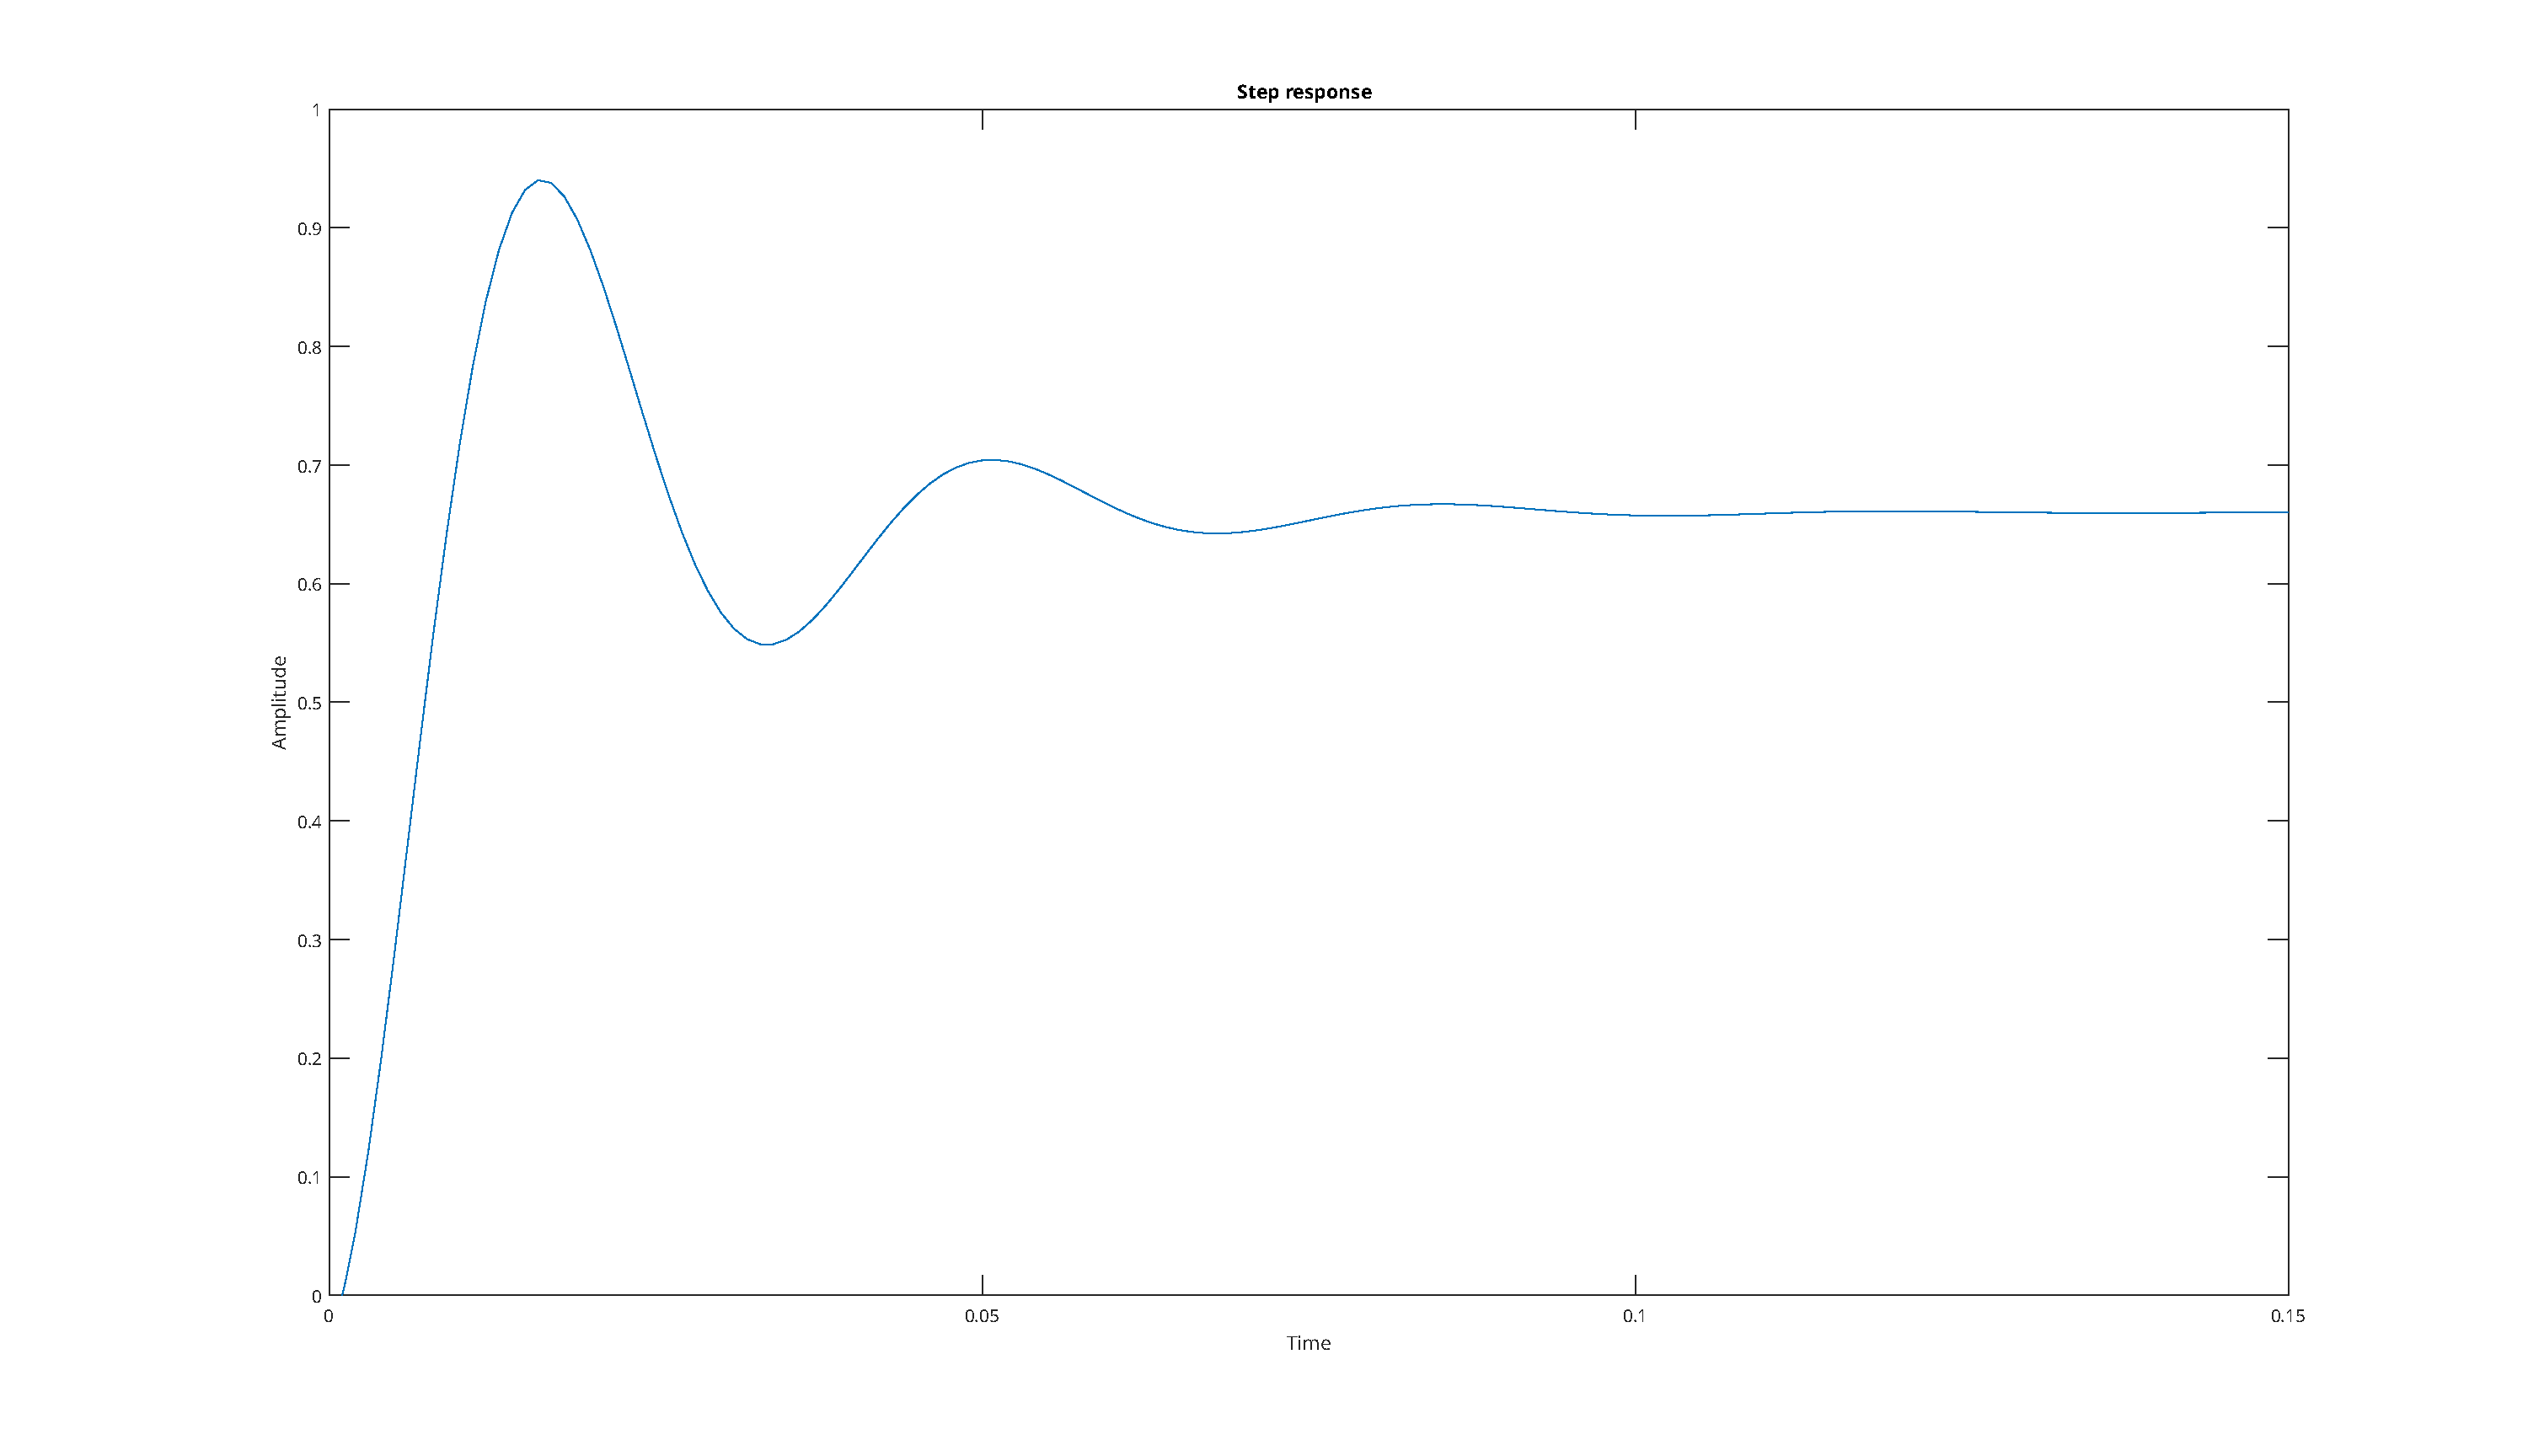
\includegraphics[width=1\linewidth]{stepResponseSystemA}
				\caption[Step response of system A]{Step response of system A}
				\label{fig:stepResponseModelA}
			\end{figure}
		
		\newpage
		\subsection{Bode plot of system A}
			Generating the bode plot is a bit more tricky. To do this, we apply a known function such as a regular sine wave, and measure the steady-state response of the system. When this procedure gets repeated for a lot of sine waves with different frequencies, we get the following bode plot (figure \ref{fig:bodePlotModelA}).  \\
		
			\begin{figure}[h]
				\centering
				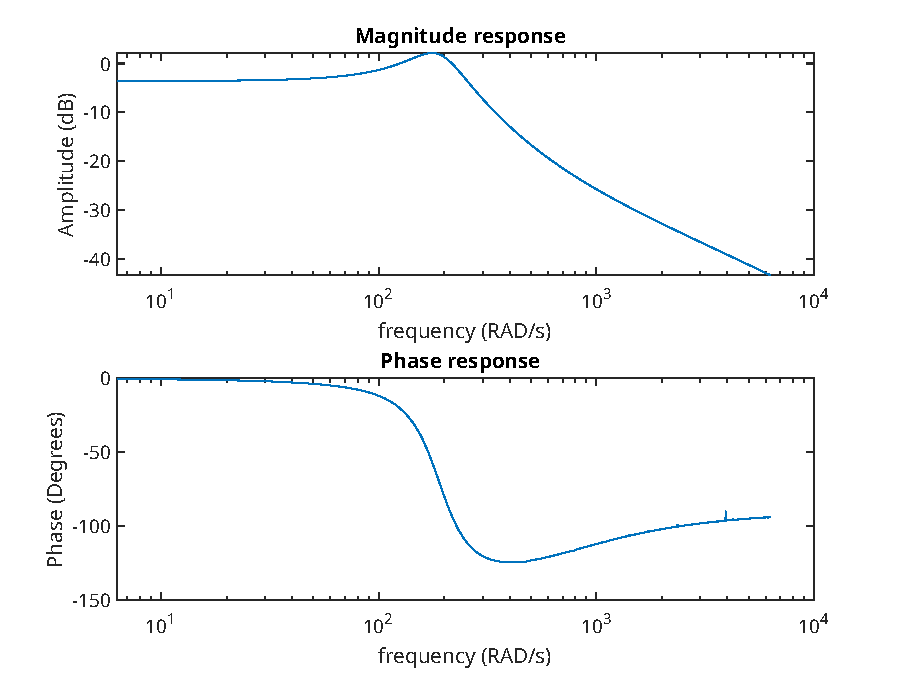
\includegraphics[width=0.7\linewidth]{generatedBodeSystemA}
				\caption[Bode of system A]{Bode plot of system A}
				\label{fig:bodePlotModelA}
			\end{figure}
			Because of the way in which we generated the bode plot, we get a few artefacts. These are especially visible  in the phase response at relatively high frequencies. However, this plot is still good enough to start an analysis of the system, in spite of the anomalies.
		
		\subsection{Discussion}
			Figures \ref{fig:stepResponseModelA} and \ref{fig:bodePlotModelA} give a lot of insight into the obfuscated system. We can now make some preliminary statements about both the stability and order of system A. 
			
			\subsubsection{Order of system A}
				\label{sec:OrderSystemA}
				We immediately notice the resonance which is present in the bode plot at approximately 200 Hz, this indicates the presence of two conjugate complex poles. This, in combination with the overshoot we see in the step response tells us we have an under damped system as well. We recognize another important point in these graphs the small crinkle in the magnitude response at approximately 500Hz. In this point, the amplitude starts descending less rapidly. This indicates the presence of a zero at around 500Hz. 
				\newline
				
				We now know the order of the system to be two. More specifically, we have a transfer function which takes the form of equation \ref{eq:generalFormTFSystemA}.
				\begin{equation}
					\label{eq:generalFormTFSystemA}
					H_A(s)=\frac{A\cdot s+B}{C\cdot s^2 + D\cdot s + E}
				\end{equation} 
				
			\newpage	
			\subsubsection{Stability of system A}
				\label{sec:StabilitySystemA}
				We first take a look at figure \ref{fig:stepResponseModelA}, the step response of system A, it tells us a few very important remarks about stability. We see an under damped system characterized by the overshoot when the step first gets applied. Critically, the system goes on to a state where the output doesn't change over time any more. This behaviour is characteristic for a stable system. If the system were to be marginally stable, we would have expected an oscillation which does not dissipate nor get out of control. For an unstable system, we expect a runaway output which - over time - goes on to reach unrealistically high values. 
				\newline
				
				Another way to analyse the stability of a system is to take a closer look at the bode plot. More specifically, we can make use of the bode plot stability criteria: both the phase and gain margin should be positive, the greater their value, the better. 
		 		
				\begin{figure}[h]
					\centering
					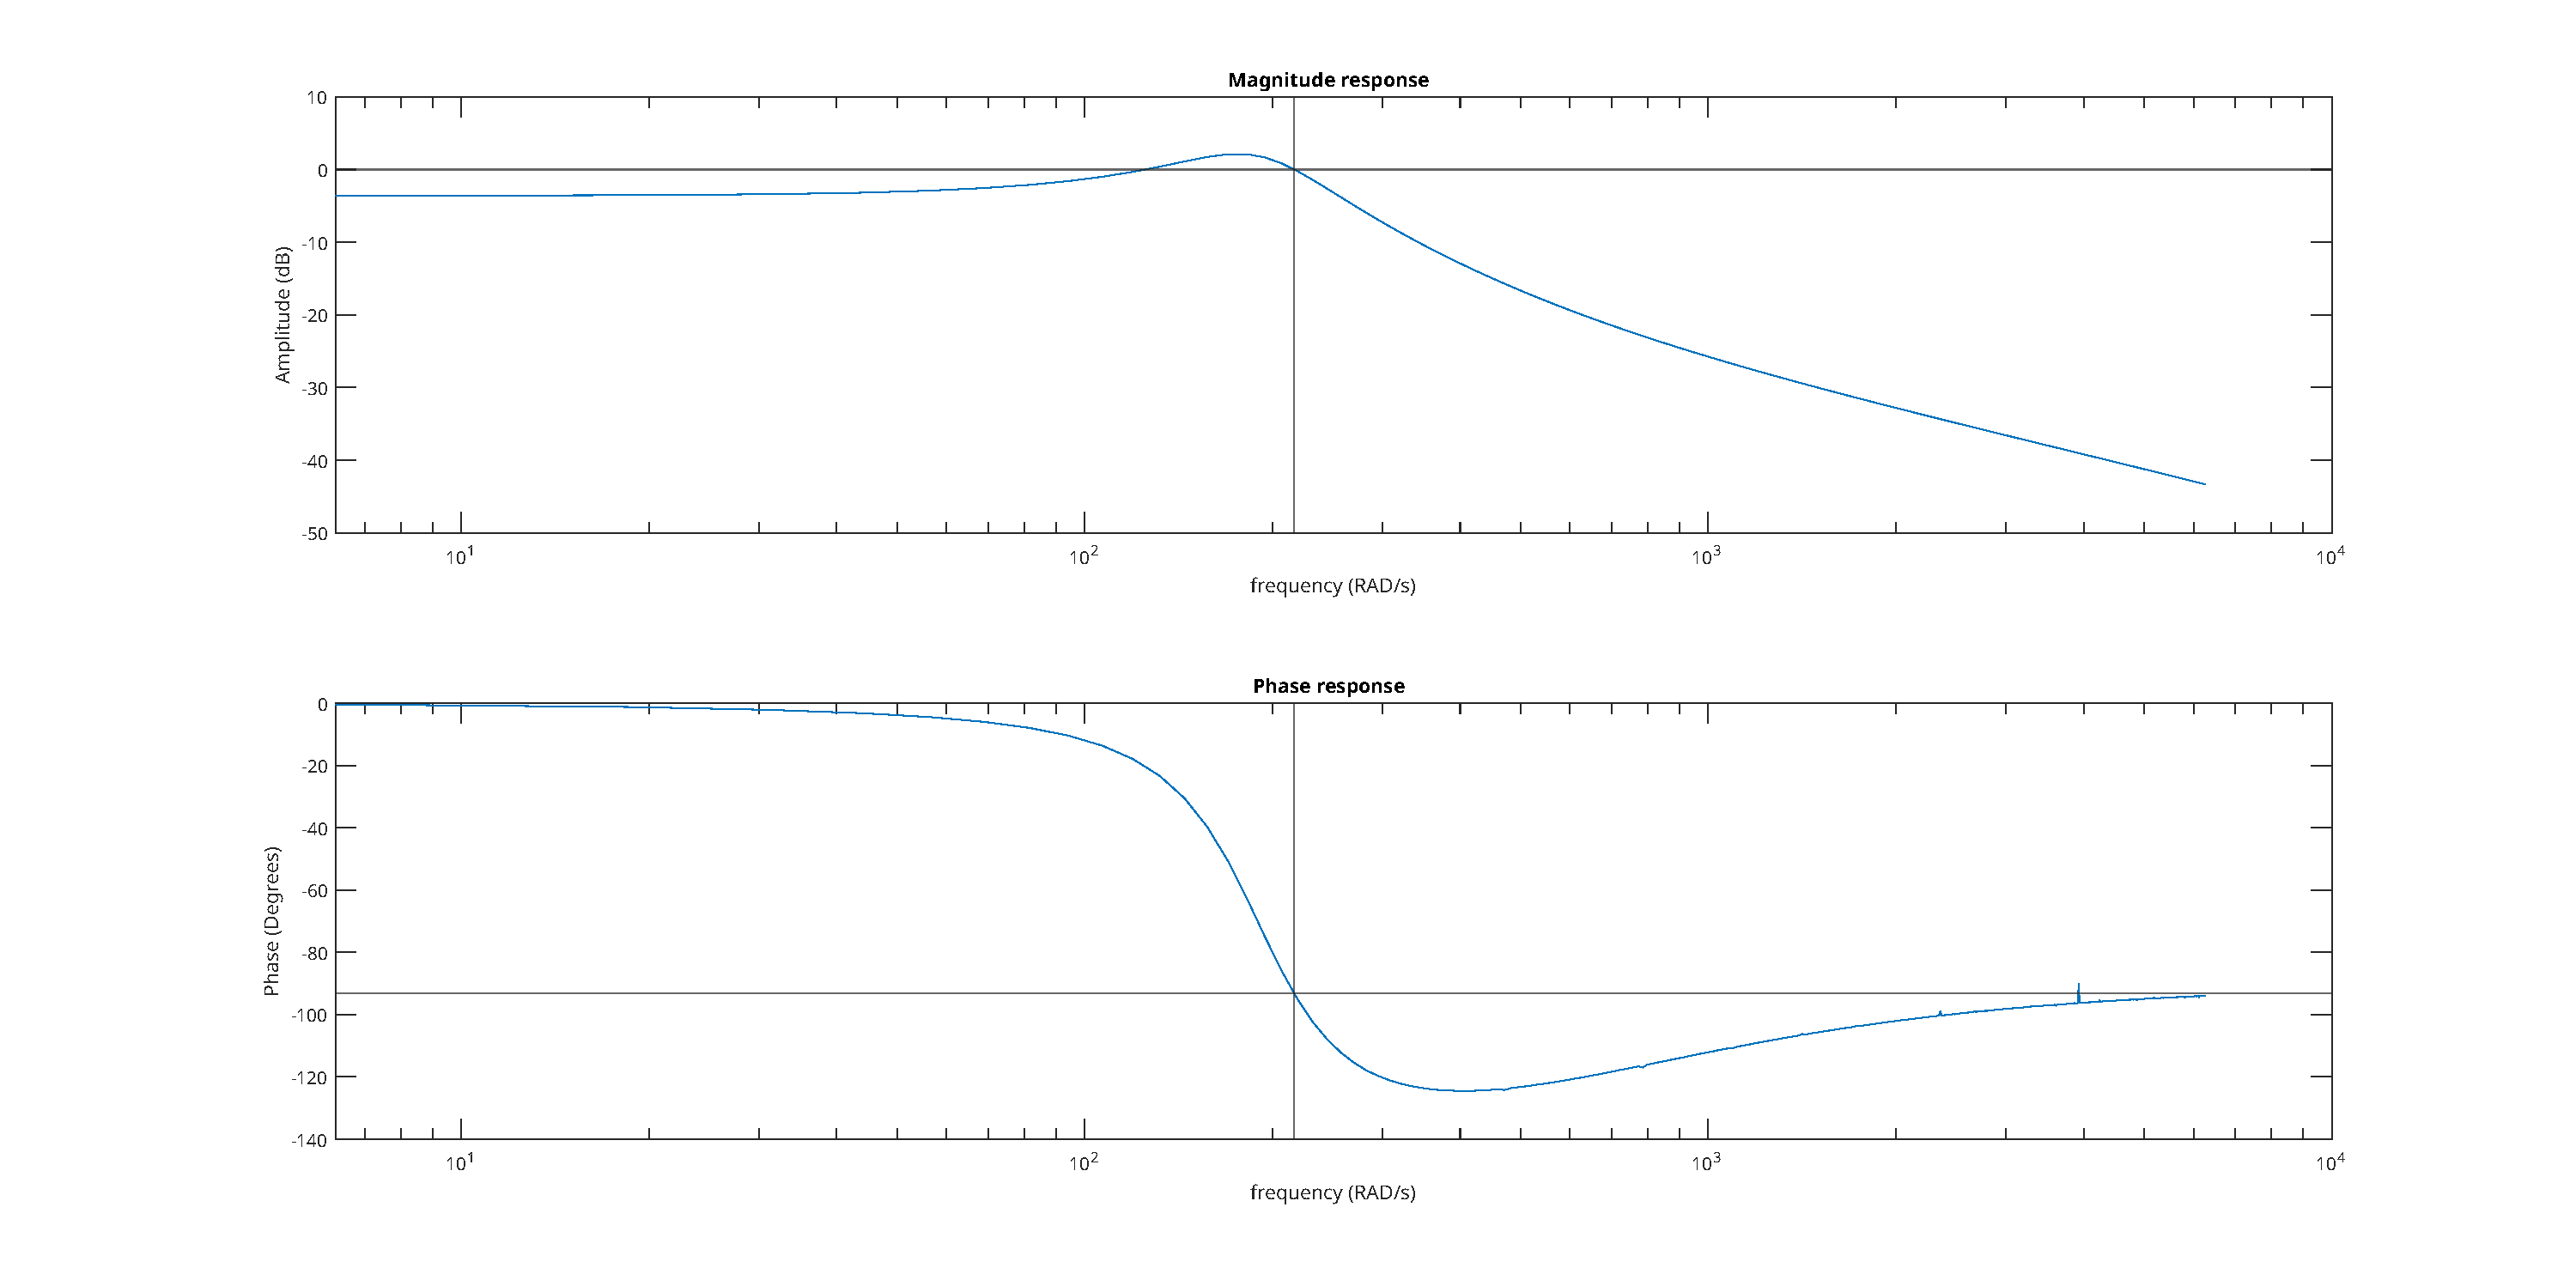
\includegraphics[width=1\linewidth]{generatedBodeSystemAStability}
					\caption[Phase margin system A]{Phase margin of system A}
					\label{fig:bodePlotModelAStability}
				\end{figure}
				
				As we can see in figure \ref{fig:bodePlotModelAStability}, the phase margin of system A is approximately 85 degrees. This is relatively good news for the stability of system A, as we have a lot of headroom for the phase margin. We can also see that we never cross the threshold of a -180 --degree shift, meaning that we can say the gain margin is infinite. Again, this is good news for the stability of system A.
				
	\newpage
	\section{Question 2: Reverse engineering of system A}
		The bode plot of system A can be used to effectively reverse engineer the transfer function of system A, we can do this by extracting key values such as the resonant frequency and the Q-factor. 
		
		\subsection{Reverse engineering method}
			In order to reverse engineer the transfer function, one can start by taking a look at the peak which forms in the amplitude response (see figure \ref{fig:bodePlotModelA}). If we divide the maximal value by the DC-gain, we get the Q-factor. 
			
			\begin{lstlisting}[style=Matlab-editor]
				[peakAmplitudeRatio, peakAmplitudeRatioIndex] = max(amplitudeRatios);
				DCamplitudeRatio = amplitudeRatios(1);
				Q = peakAmplitudeRatio/DCamplitudeRatio;
			\end{lstlisting}
			
			Having found the Q-factor, it is trivial to calculate the damping $\zeta$, as it can be obtained through the use of a simple formula $\zeta = \frac{1}{2\cdot Q}$. This now enables us to find the natural frequency $\omega_0$ of system A, due to the fact we also know the frequency at which the peak occurs. 
			
			\begin{lstlisting}[style=Matlab-editor]
				peakFrequency = frequency(peakAmplitudeRatioIndex);
				naturalFrequency = peakFrequency/(sqrt(1-2*zeta^2));
			\end{lstlisting}
			
			The last parameter needed to characterize our system, is $\tau_z$.  Unfortunately, there is no wonderful method for extracting this parameter from the bode plot other than making an educated guess.  We know there must be a zero in the system because of the change at around 500Hz mentioned in section \ref{sec:OrderSystemA}.  Using the approximate location of this zero, we can make our guess using the following MATLAB code:
			
			\begin{lstlisting}[style=Matlab-editor]
				zeroGuess = 540;  % here is a guess of what the value is for the zero in the system
				tau_z = 1/zeroGuess;
			\end{lstlisting}
			
			Plugging these parameters into formula \ref{eq:TransferFunctionTemplate}, gives us the reverse engineered transfer function we wanted (equation \ref{eq:TransferFunctionSystemA}). 
			
			\begin{align}
				\label{eq:TransferFunctionTemplate}
				H(s)&=\frac{K_{DC}\omega_0\cdot(\tau_zs+1)}{s^2+2\zeta\omega_0s+\omega_0^2}\\
				\label{eq:TransferFunctionSystemA}
				H(s)&= \frac{40.66s + 21960}{s^2+94.42s+33240}
			\end{align}
			
			\begin{lstlisting}[style=Matlab-editor]
				numerator = (DCamplitudeRatio * naturalFrequency^2).*[tau_z, 1];
				denominator = [1, 2*zeta*naturalFrequency, naturalFrequency^2];
				REsystemA = tf(numerator, denominator);
			\end{lstlisting}
		
		\newpage	
		\subsection{Comparison of the original and reverse engineer}
			Having found a potential transfer function, we now compare its behaviour against the unknown system A. We can start by plotting the step response for both and overlaying them on each other (see figure \ref{fig:StepCompared}).\\ 
			
			\begin{figure}[h]
				\centering
				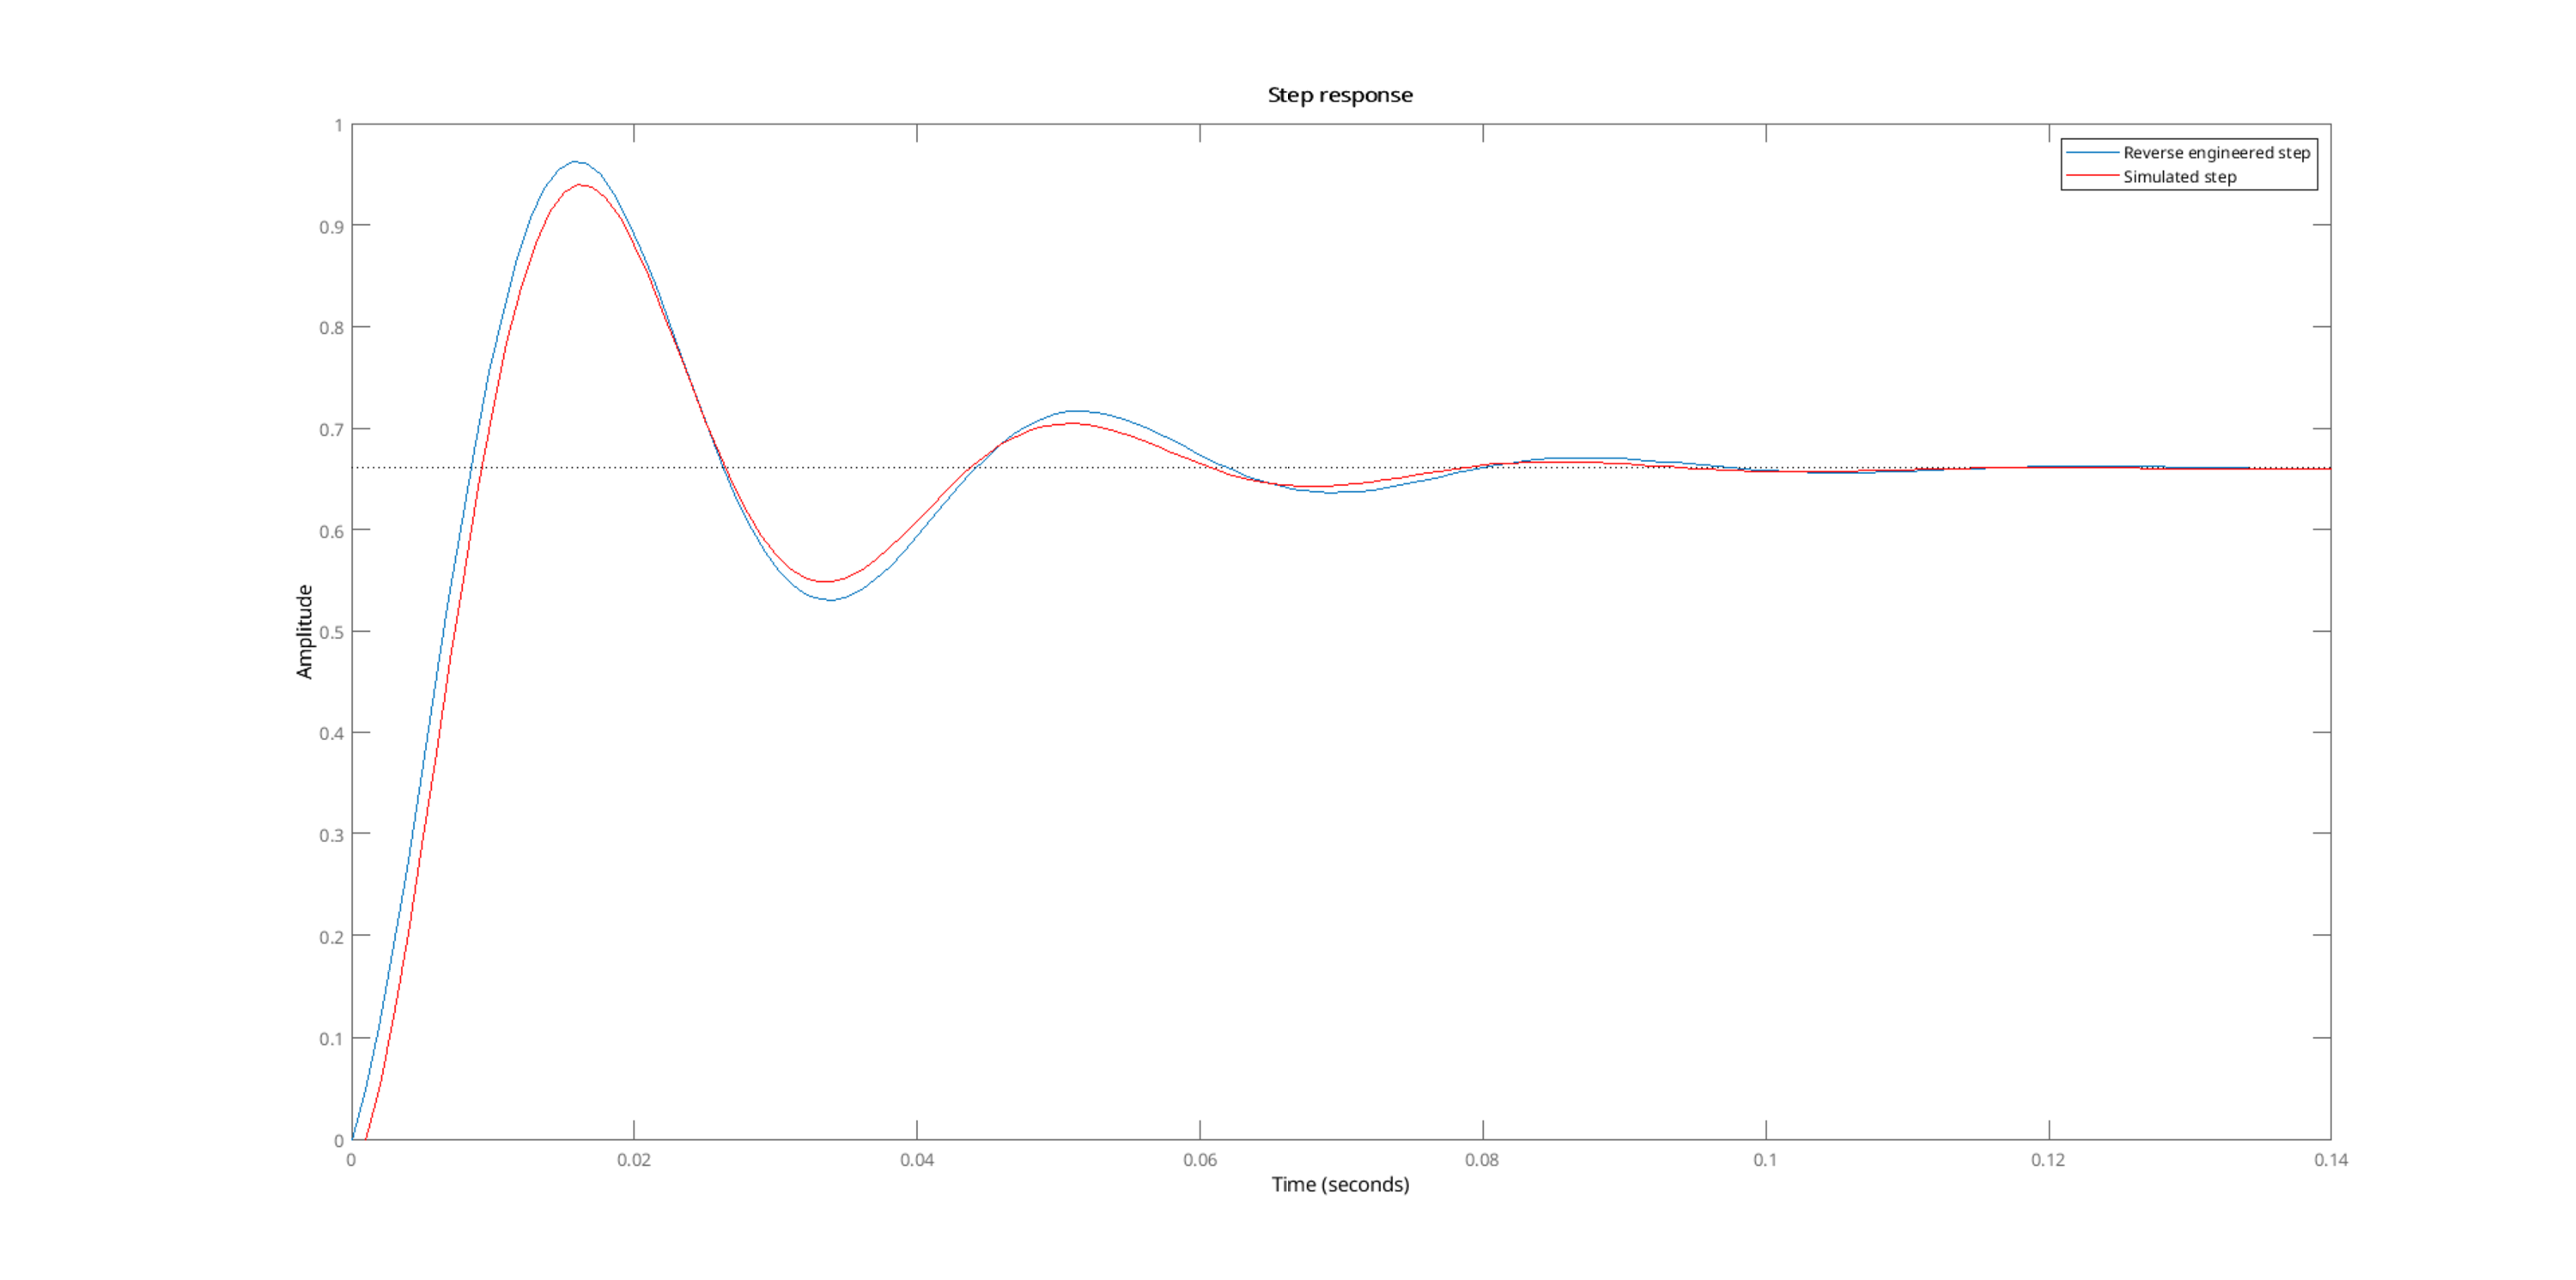
\includegraphics[width=1\linewidth]{StepCompared}
				\caption[Comparing step responses]{Comparison of system A with the reverse engineered step response}
				\label{fig:StepCompared}
			\end{figure}
			
			Although the responses aren't exactly the same, we can see they are quite akin to each other. This, in practice, means that our revere engineer is of a decent quality. To further prove our point, we can take a look at the bode plots of both systems (figure \ref{fig:BodeCompared}). 
			
			\begin{figure}[h]
				\centering
				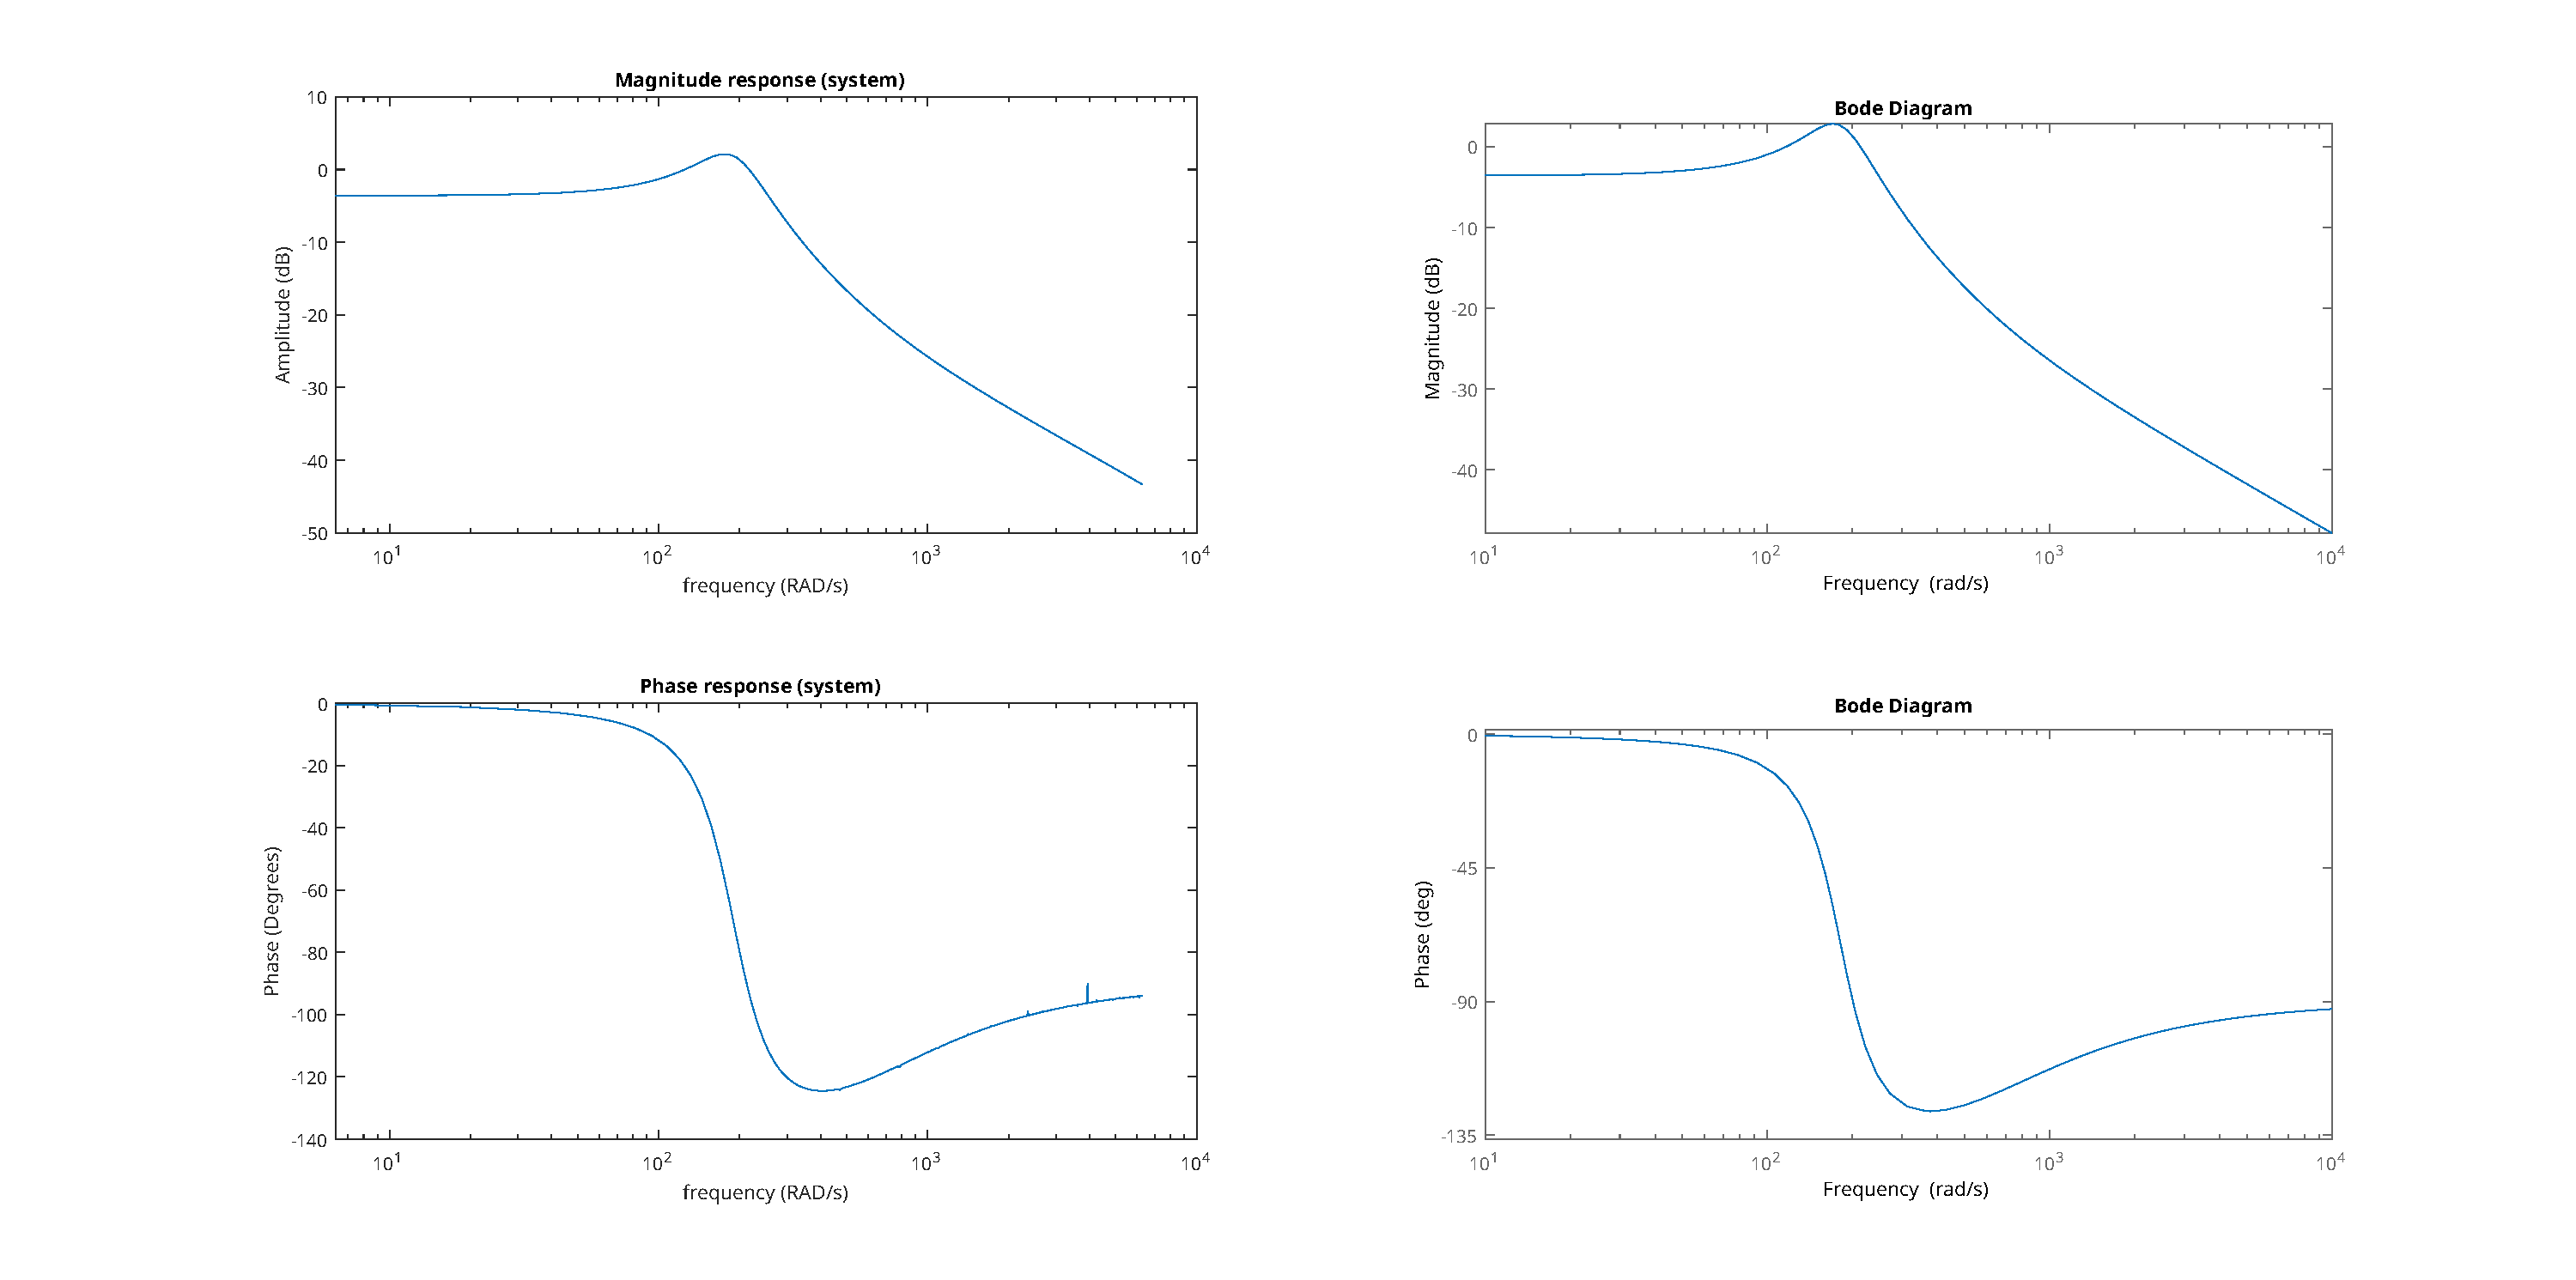
\includegraphics[width=1\linewidth]{BodeCompare}
				\caption[Comparing bode plots]{Comparison of system A with the reverse engineered bode plot}
				\label{fig:BodeCompared}
			\end{figure}
			
		\newpage
		\subsection{Reflection}
			Visually, we can see both the reverse engineer and the original are pretty alike. There are of course differences which are most easily spotted in the step response. However, we can still accept the results as `good enough'. In order to improve the accuracy of the transfer function, we could increase the resolution of our bode plot, i.e. sample the obfuscated model at more points. This would increase the accuracy of the \matlab{peakAmplitudeRatio} and the \matlab{peakAmplitudeRatioIndex}, which is beneficial for finding $\zeta$ and $\omega_0$.  The largest improvement however, could be found by finding a more accurate guess for the location of our zero. This step is by far the most improvised part of reverse engineering the transfer function.
	\newpage
	\section{Question 3: Analysis of system B}
		\subsection{Stability of system B}
			Looking at the sub figures of figure \ref{fig:stabilitySystemB}, it is immediately  obvious that system B is unstable. Firstly, in the rlocus plot shown in figure \ref{fig:rlocusSystemB} reveals that we have poles with positive real parts. This is indicative of an unstable system. Furthermore, we see a negative gain margin in figure \ref{fig:marginSystemB}. This is another big indicator for instability, as it violates the bode stability criterion. Finally, the step response of system B (figure \ref{fig:stepSystemB}) confirms the observations made before, we see a system which can not by any stretch of the imagination be called stable.  
	
			\begin{figure}[h]
				\centering
				\begin{subfigure}{.5\textwidth}
					\centering
					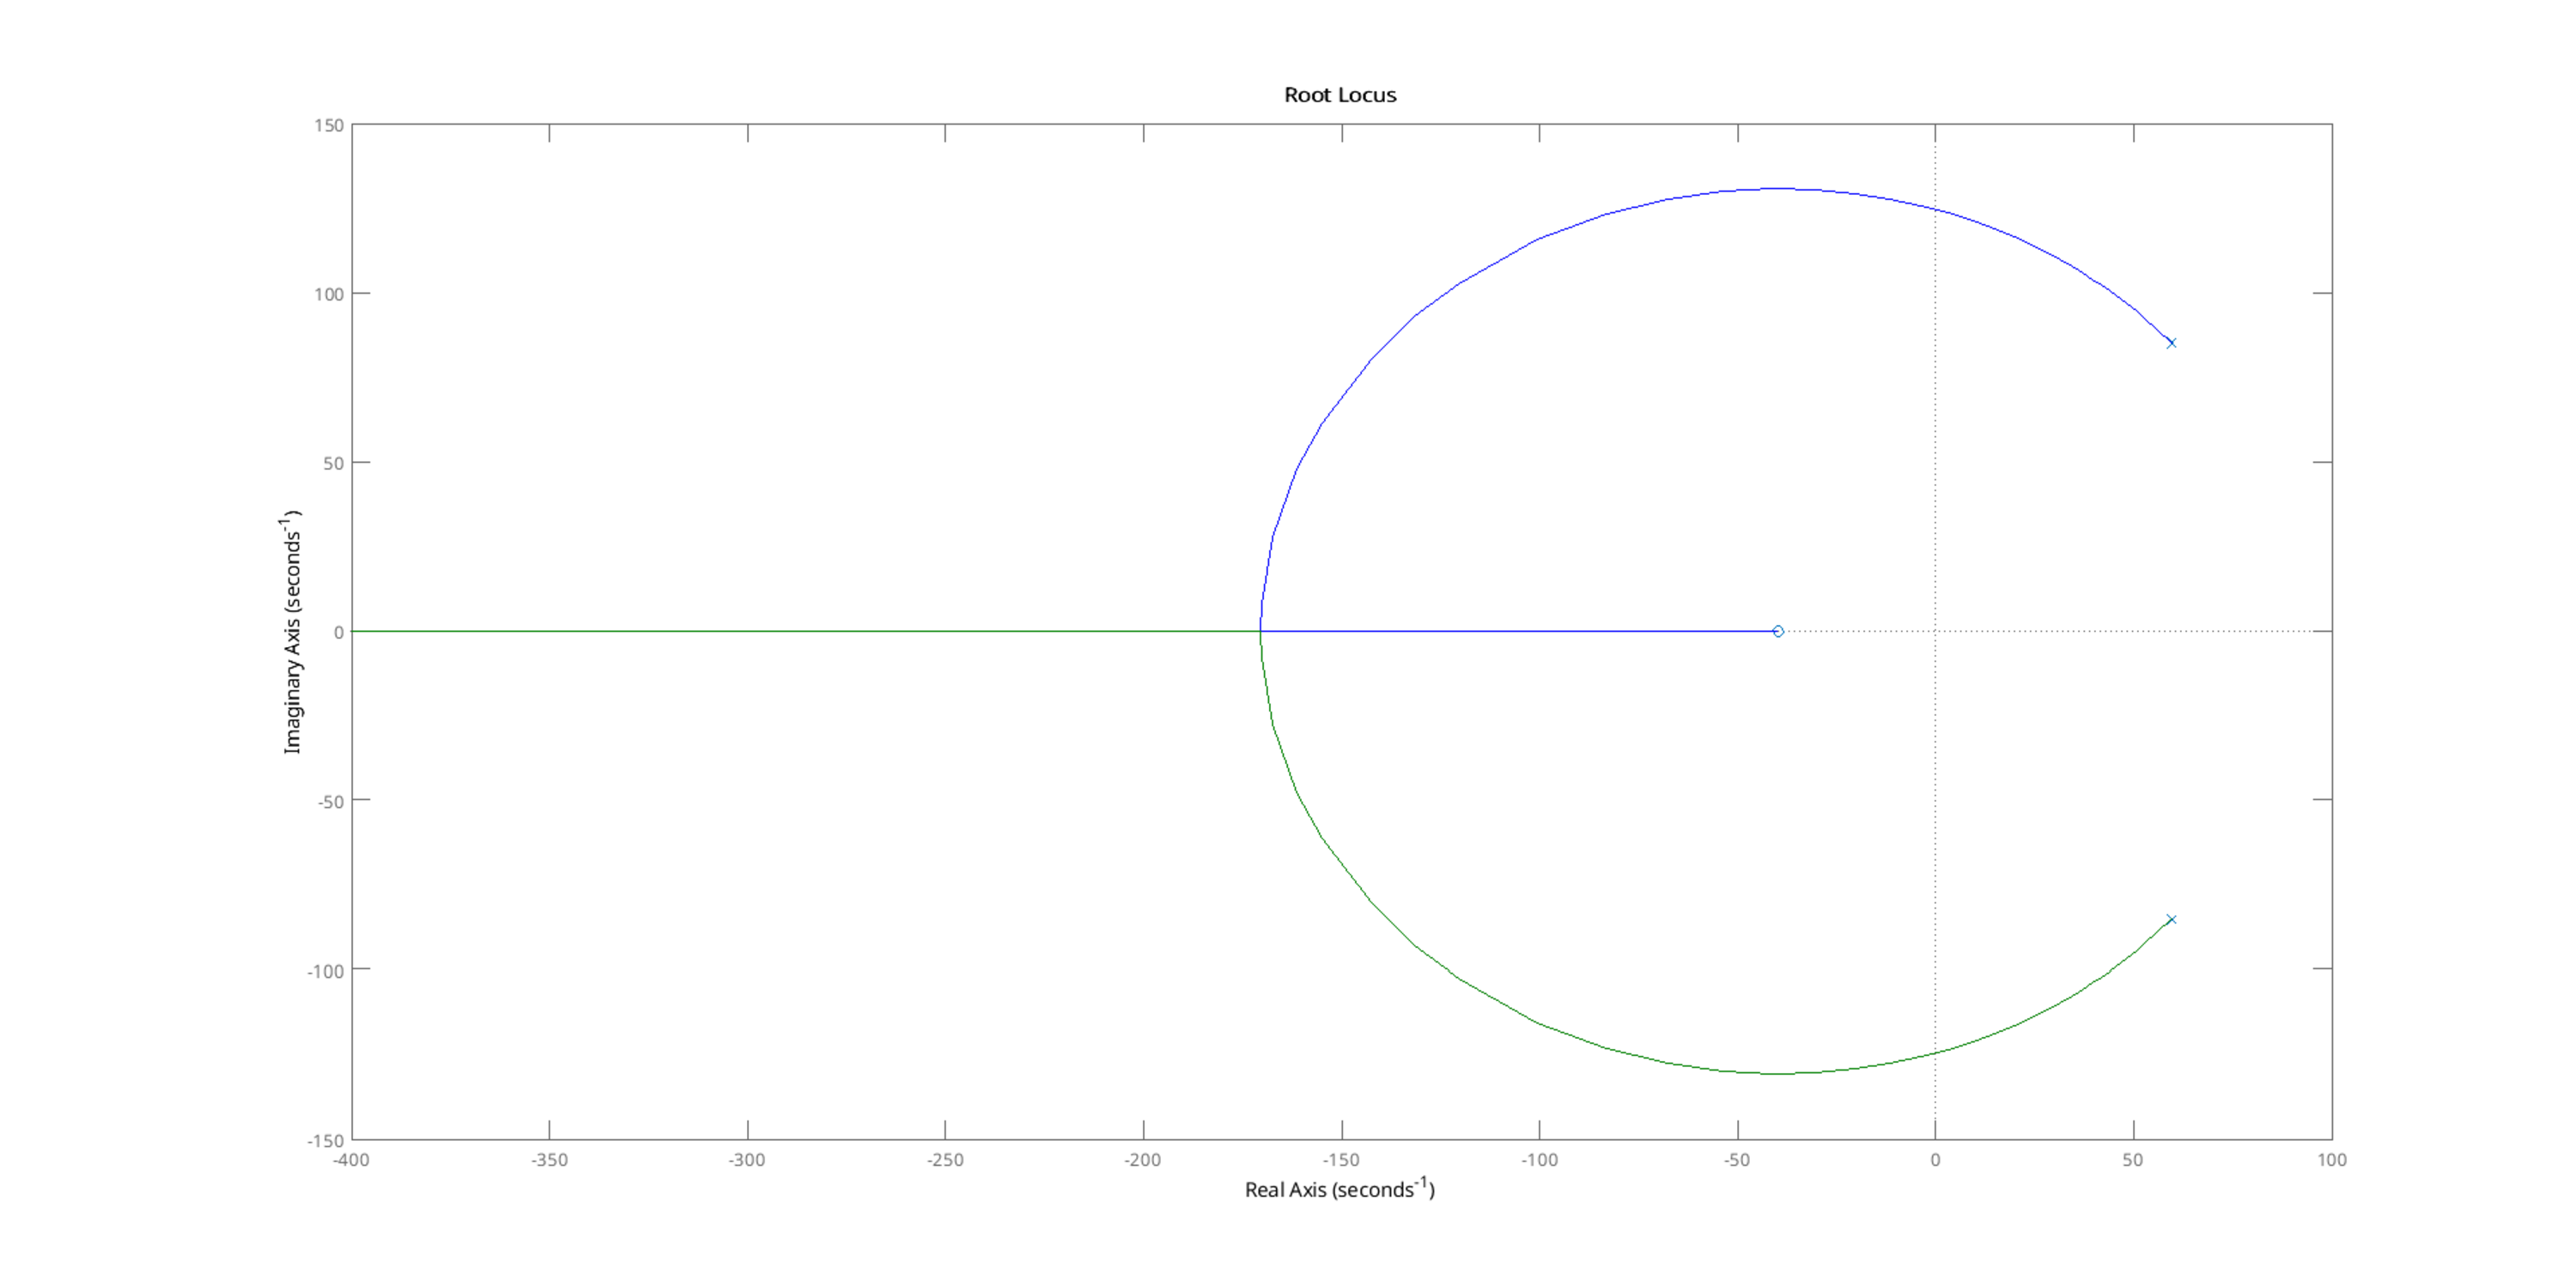
\includegraphics[width=1\linewidth]{rlocusSystemB}
					\caption[rlocus system B]{rlocus plot of system B}
					\label{fig:rlocusSystemB}
				\end{subfigure}%
				\begin{subfigure}{.5\textwidth}
					\centering
					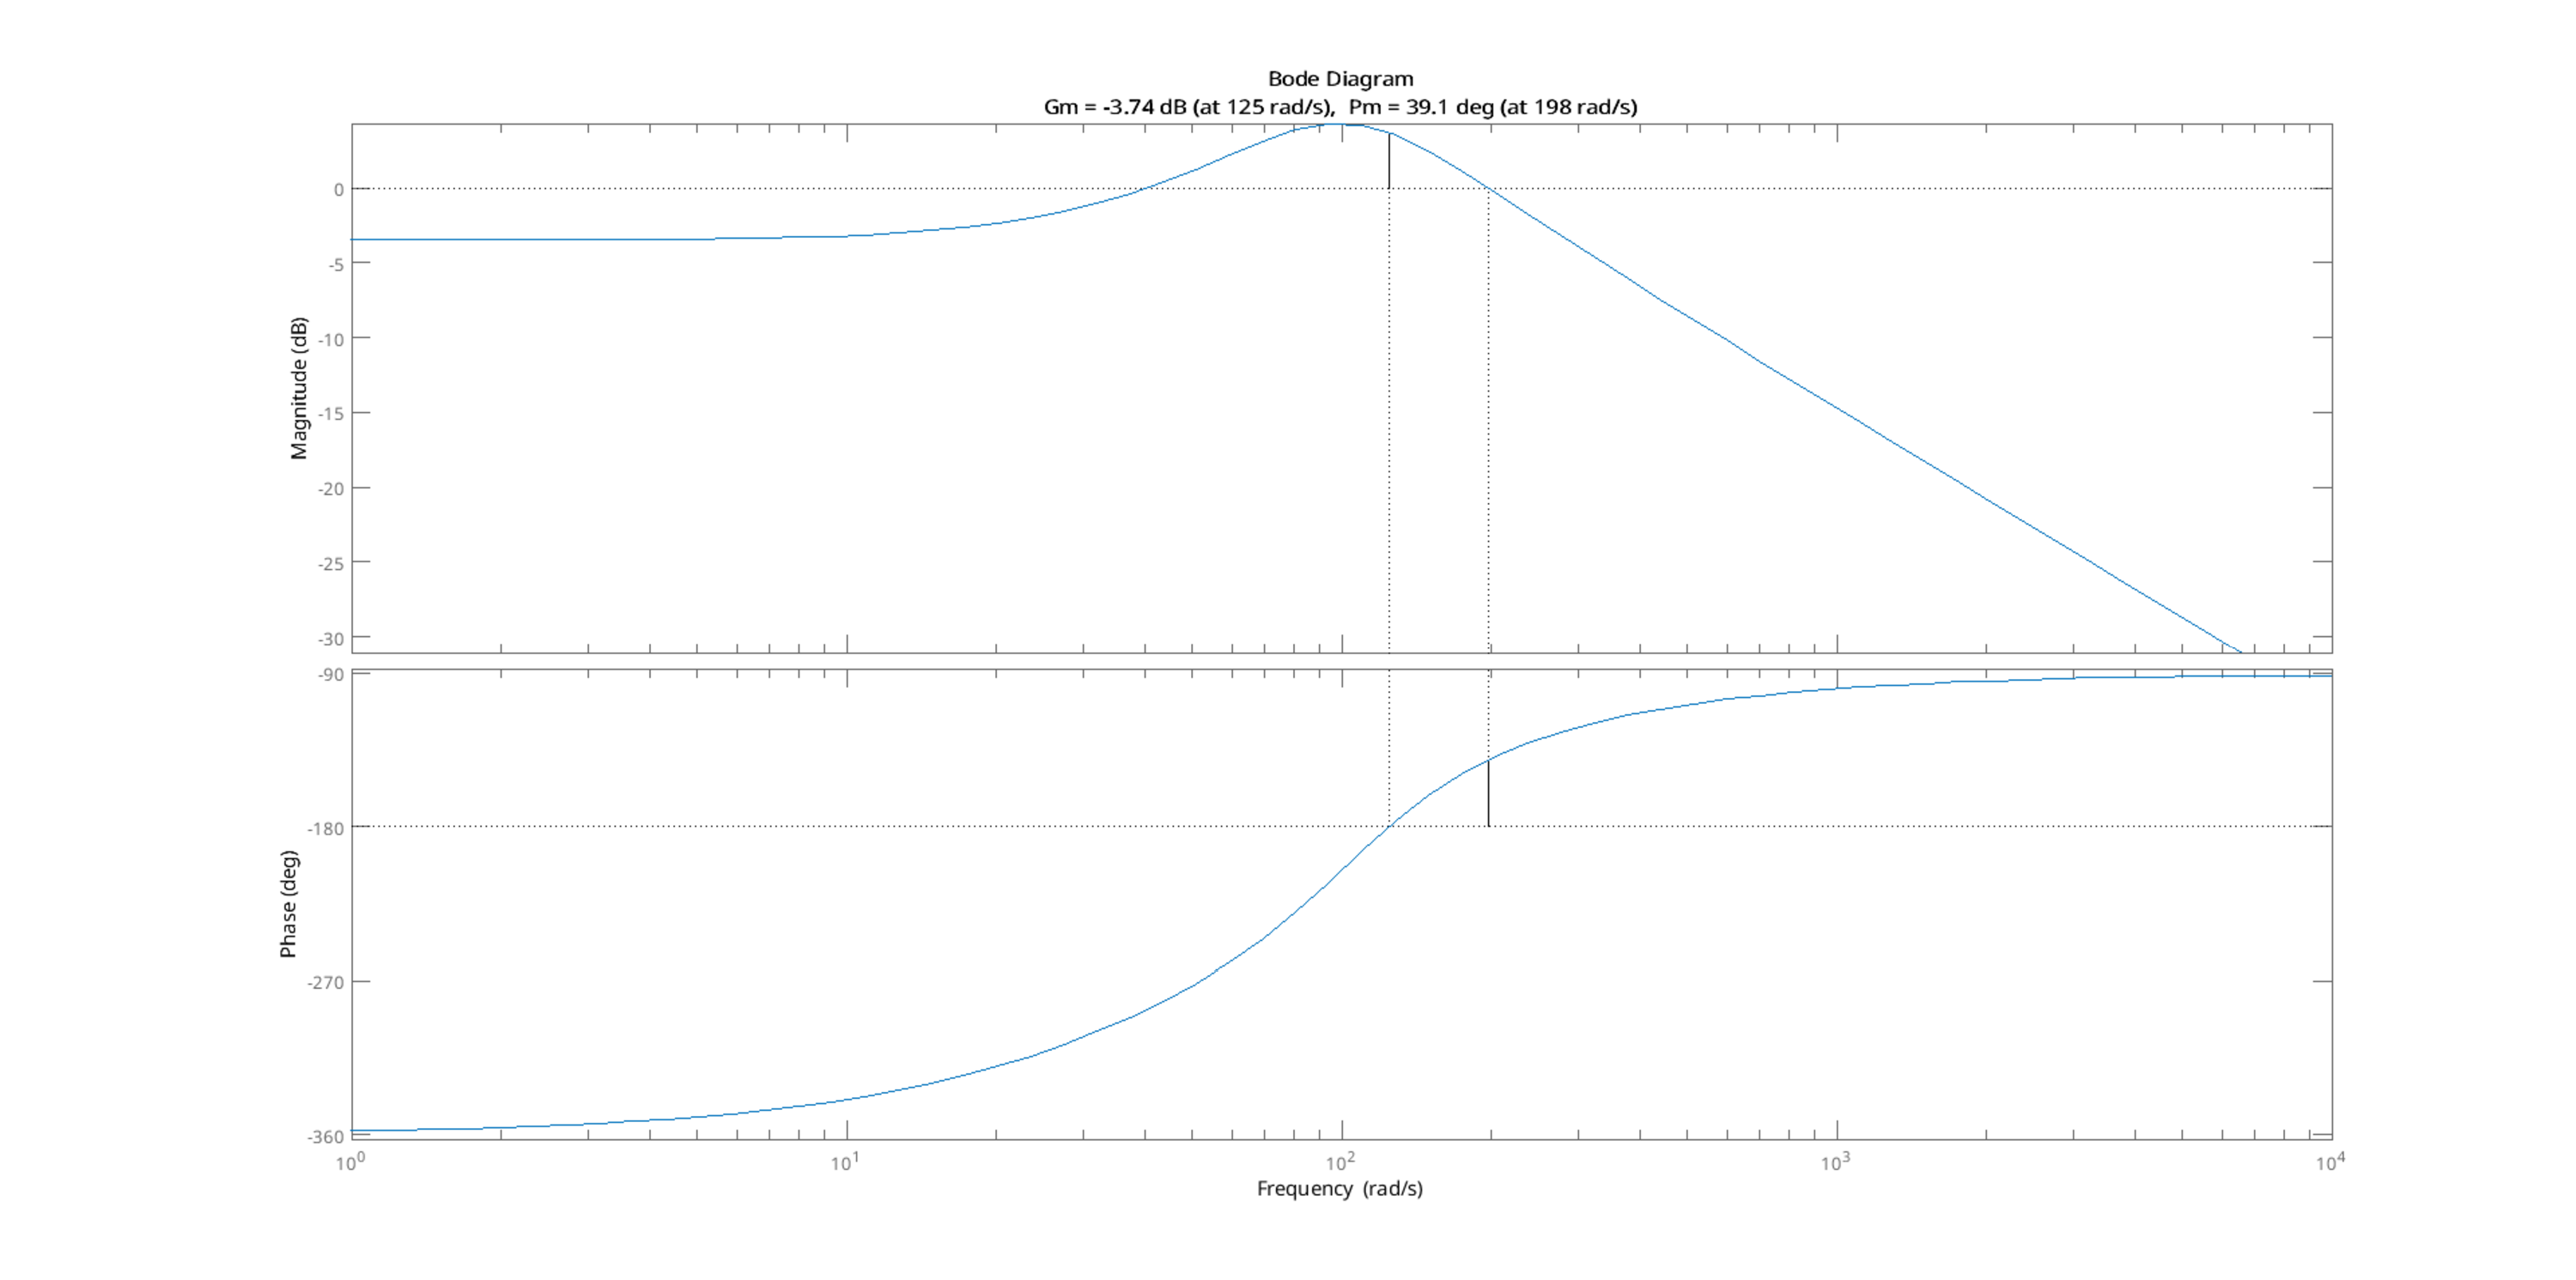
\includegraphics[width=1\linewidth]{marginSystemB}
					\caption[margin system B]{Margin plot of system B}
					\label{fig:marginSystemB}
				\end{subfigure}
				\caption{Stability of system B}
				\label{fig:stabilitySystemB}
			\end{figure}
			
			\begin{figure}[h]
				\centering
				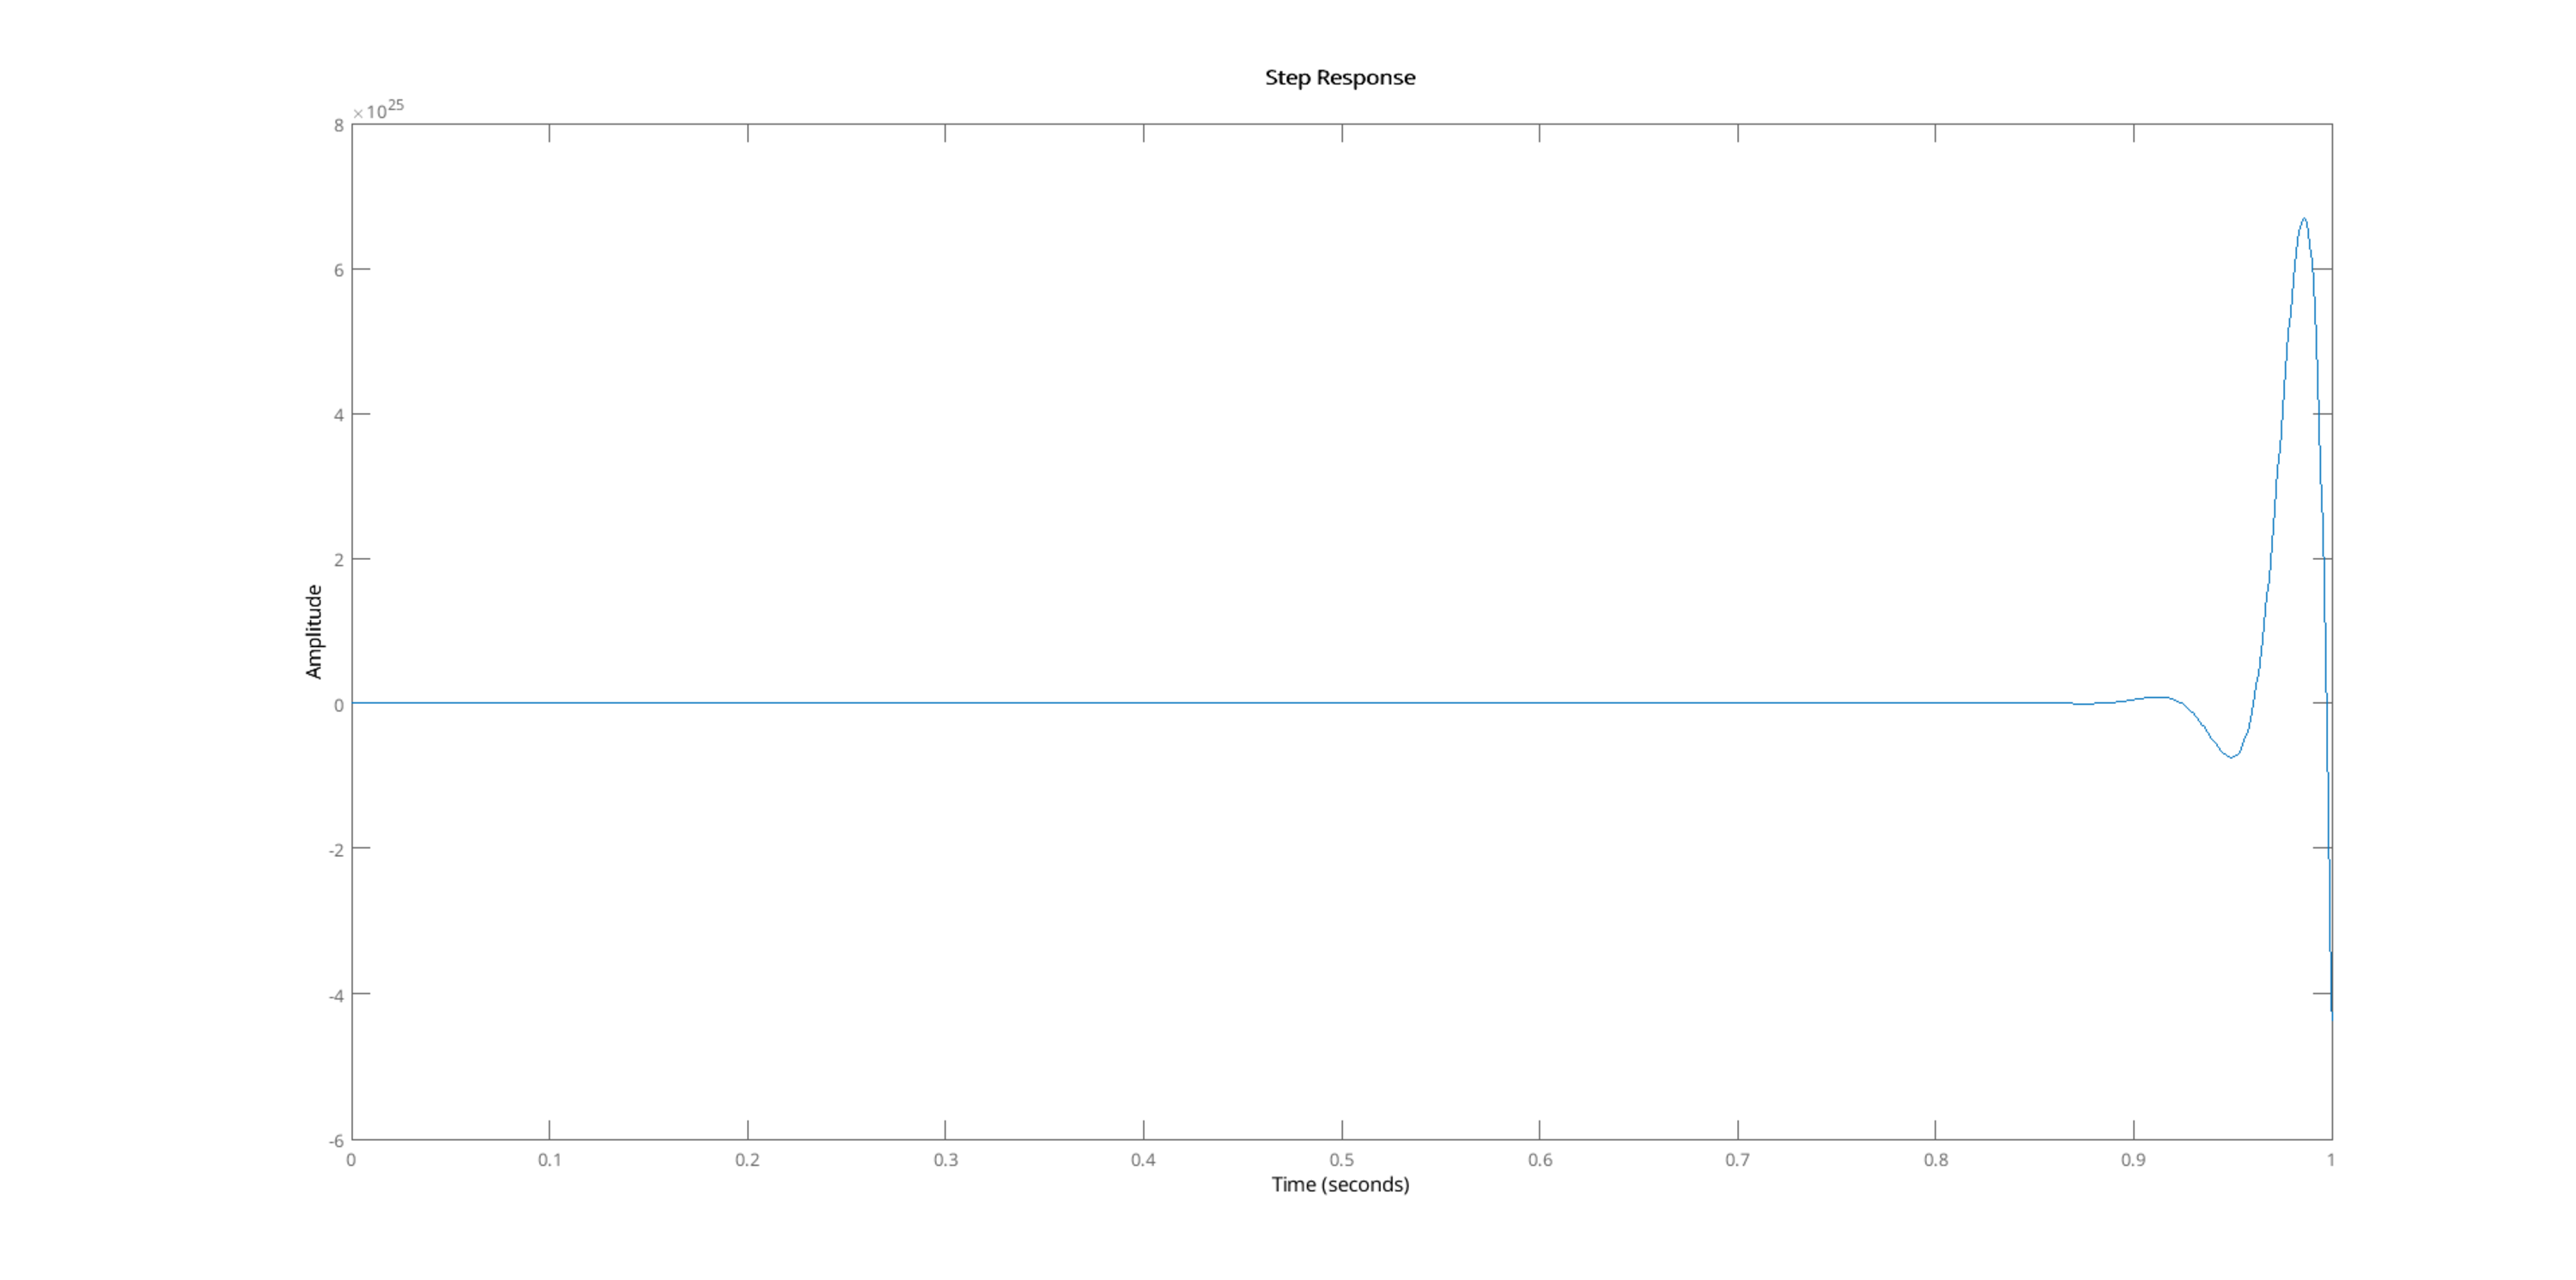
\includegraphics[width=0.7\linewidth]{stepSystemB}
				\caption[step system B]{Step response of system B}
				\label{fig:stepSystemB}
			\end{figure}
		
		\newpage
		\subsection{Stabilizing system B with a P controller}
			\label{sec:PcontrollerSystemB}
			We can stabilize the system with a simple addition of a P controller as seen in figure \ref{fig:PcontrollerSystemB}. The sensor has been set to have a transfer function equal to $\frac{1}{1}$. The only thing left to do is dial in  the right value for $K$ So that we get a stable system. To find this, we can have a closer look at the rlocus plot shown in figure \ref{fig:rlocusSystemB}. This tells us that we have a stable system when applying a gain of about \num{0.64}. Through some trail and error, we can find that the system gets pretty close to marginally stable for a $K$ of \num{0.6502732}. This results in a step response seen in figure \ref{fig:stepControlledB}. 
			\begin{figure}[h]
				\centering
				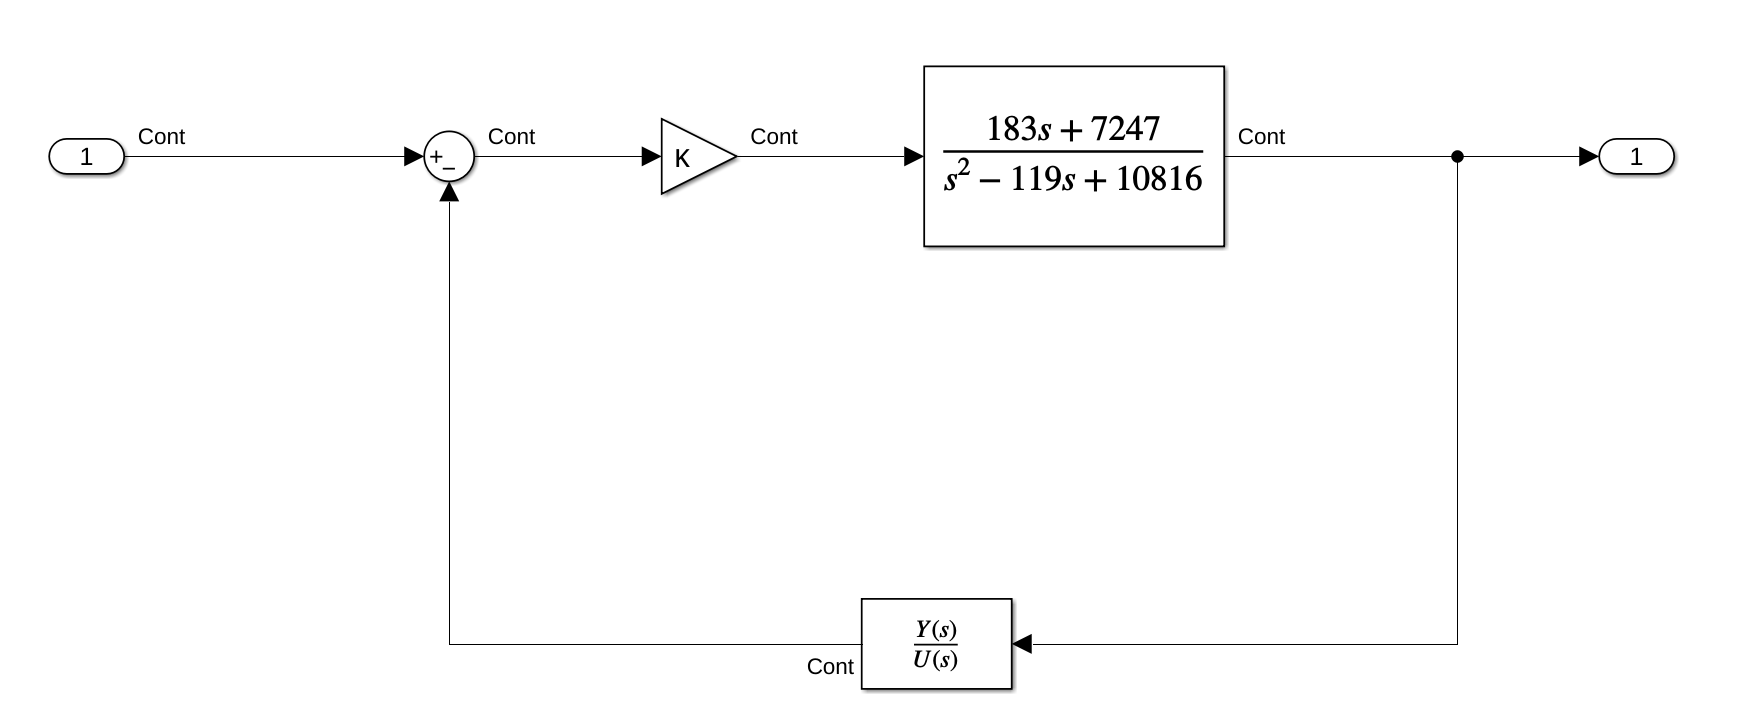
\includegraphics[width=0.7\linewidth]{PcontrollerSystemB}
				\caption[P controller system B]{P controller for system B}
				\label{fig:PcontrollerSystemB}
			\end{figure}
			\begin{figure}[h]
				\centering
				\begin{subfigure}{.5\textwidth}
					\centering
					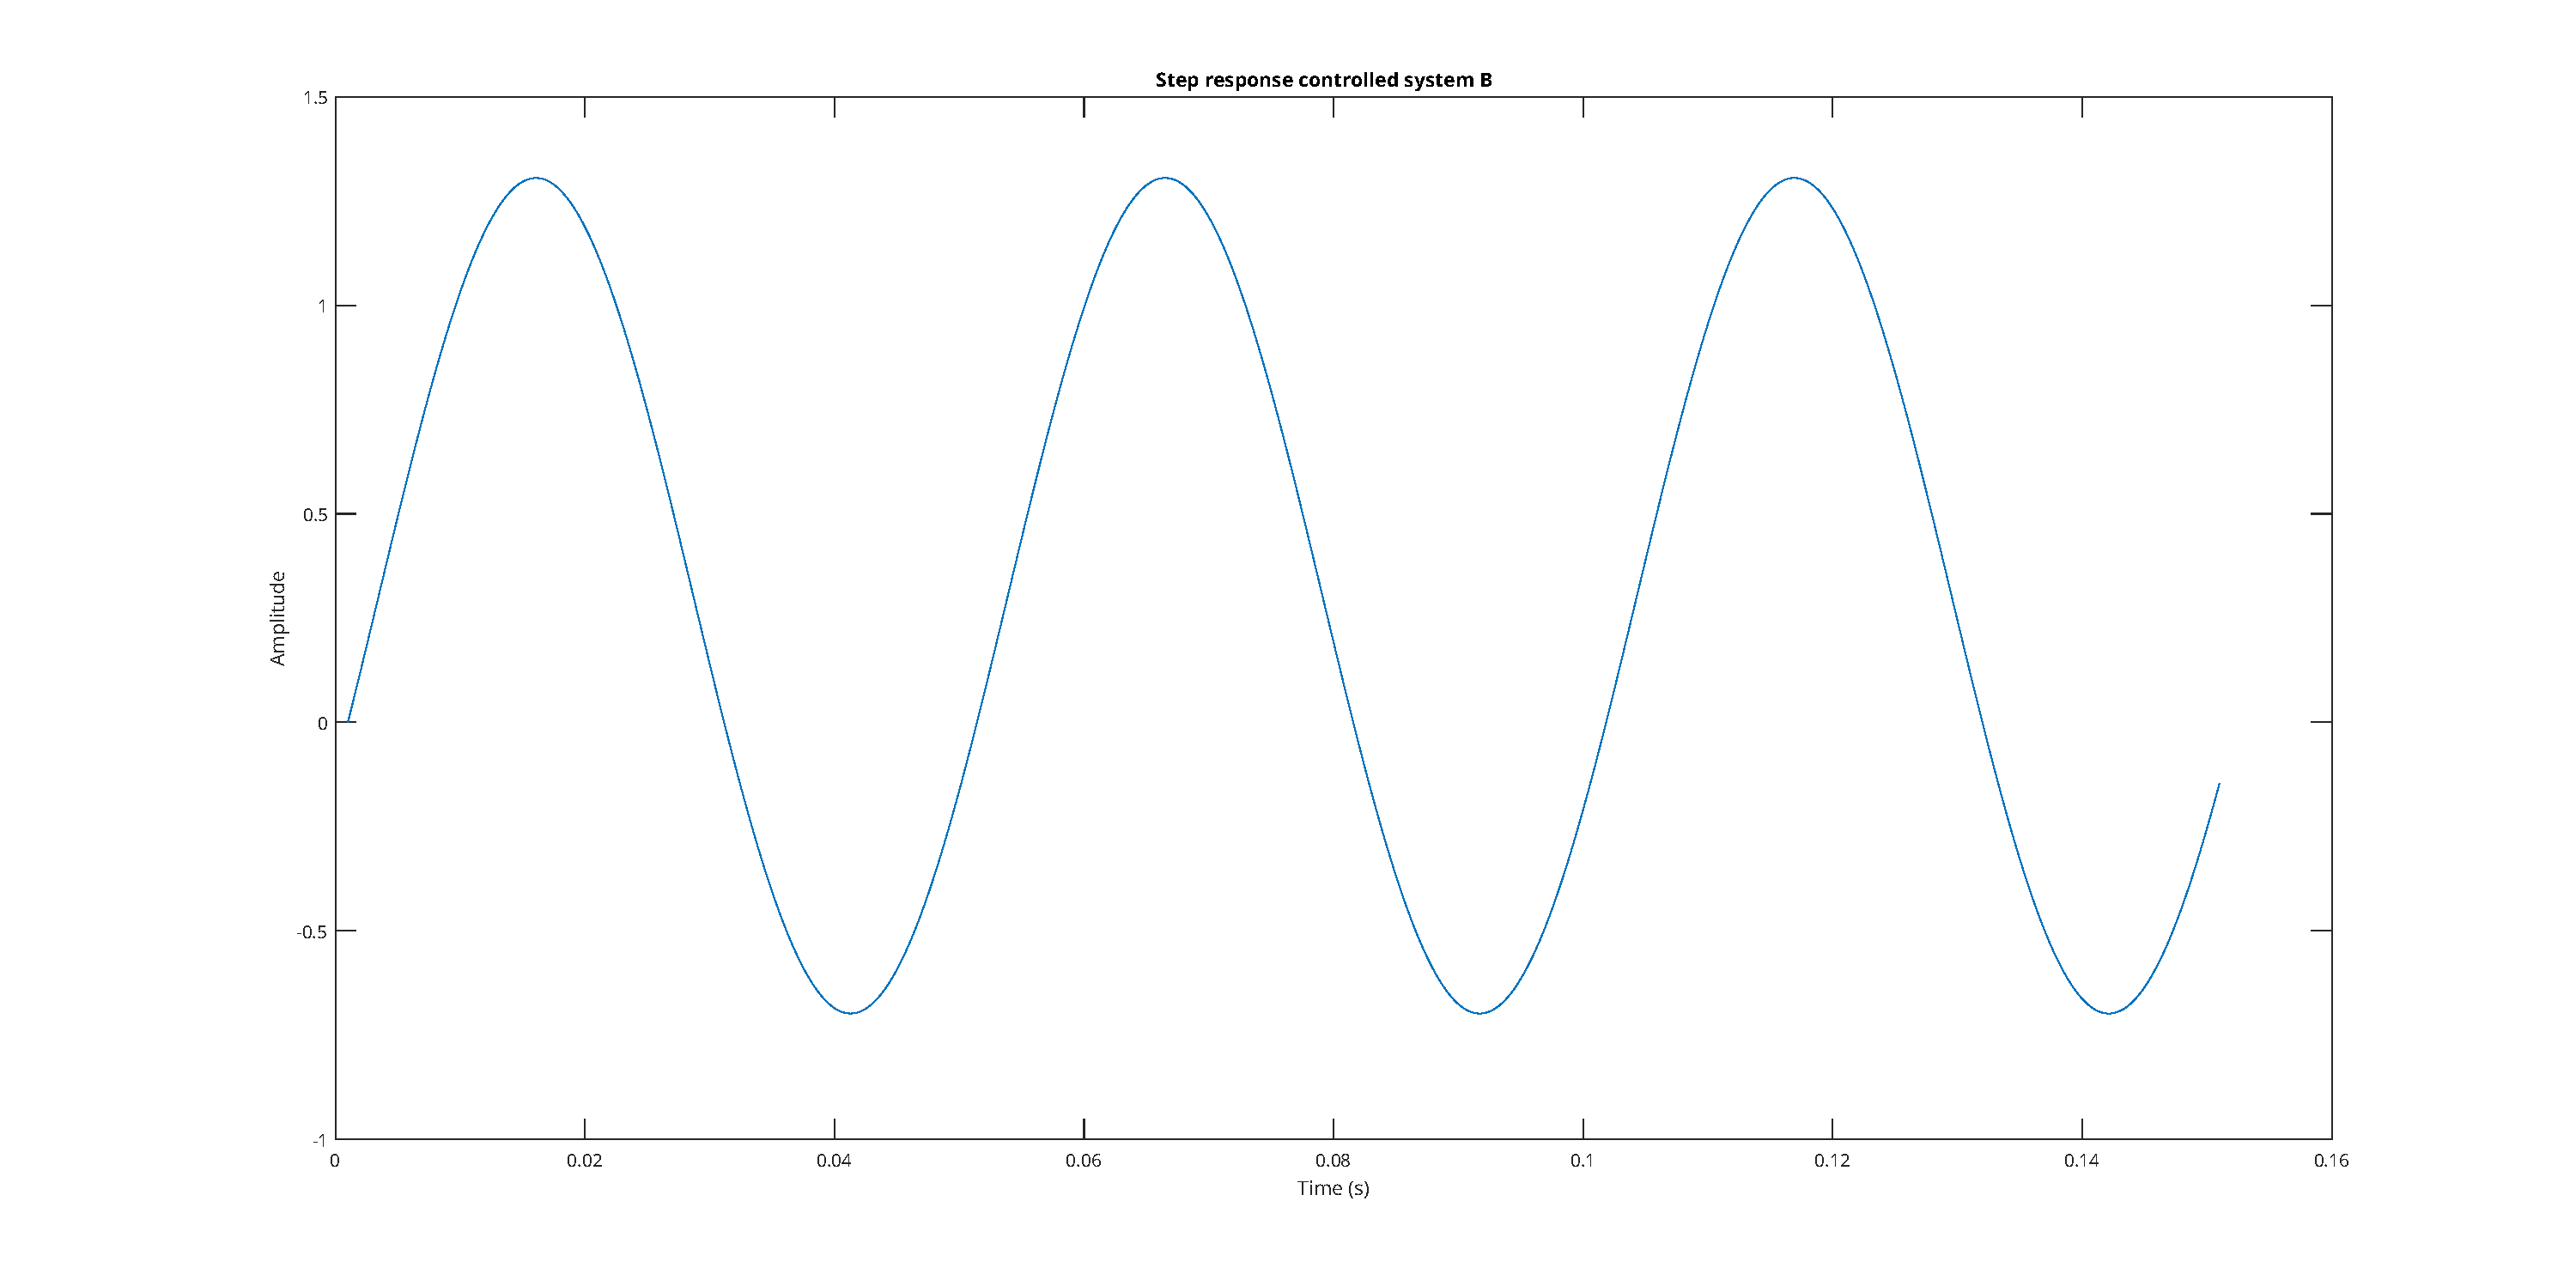
\includegraphics[width=1\linewidth]{stepControlledSystemBShort}
					\caption[step marginal system B short]{short time period}
					\label{fig:stepControlledBShort}
				\end{subfigure}%
				\begin{subfigure}{.5\textwidth}
					\centering
					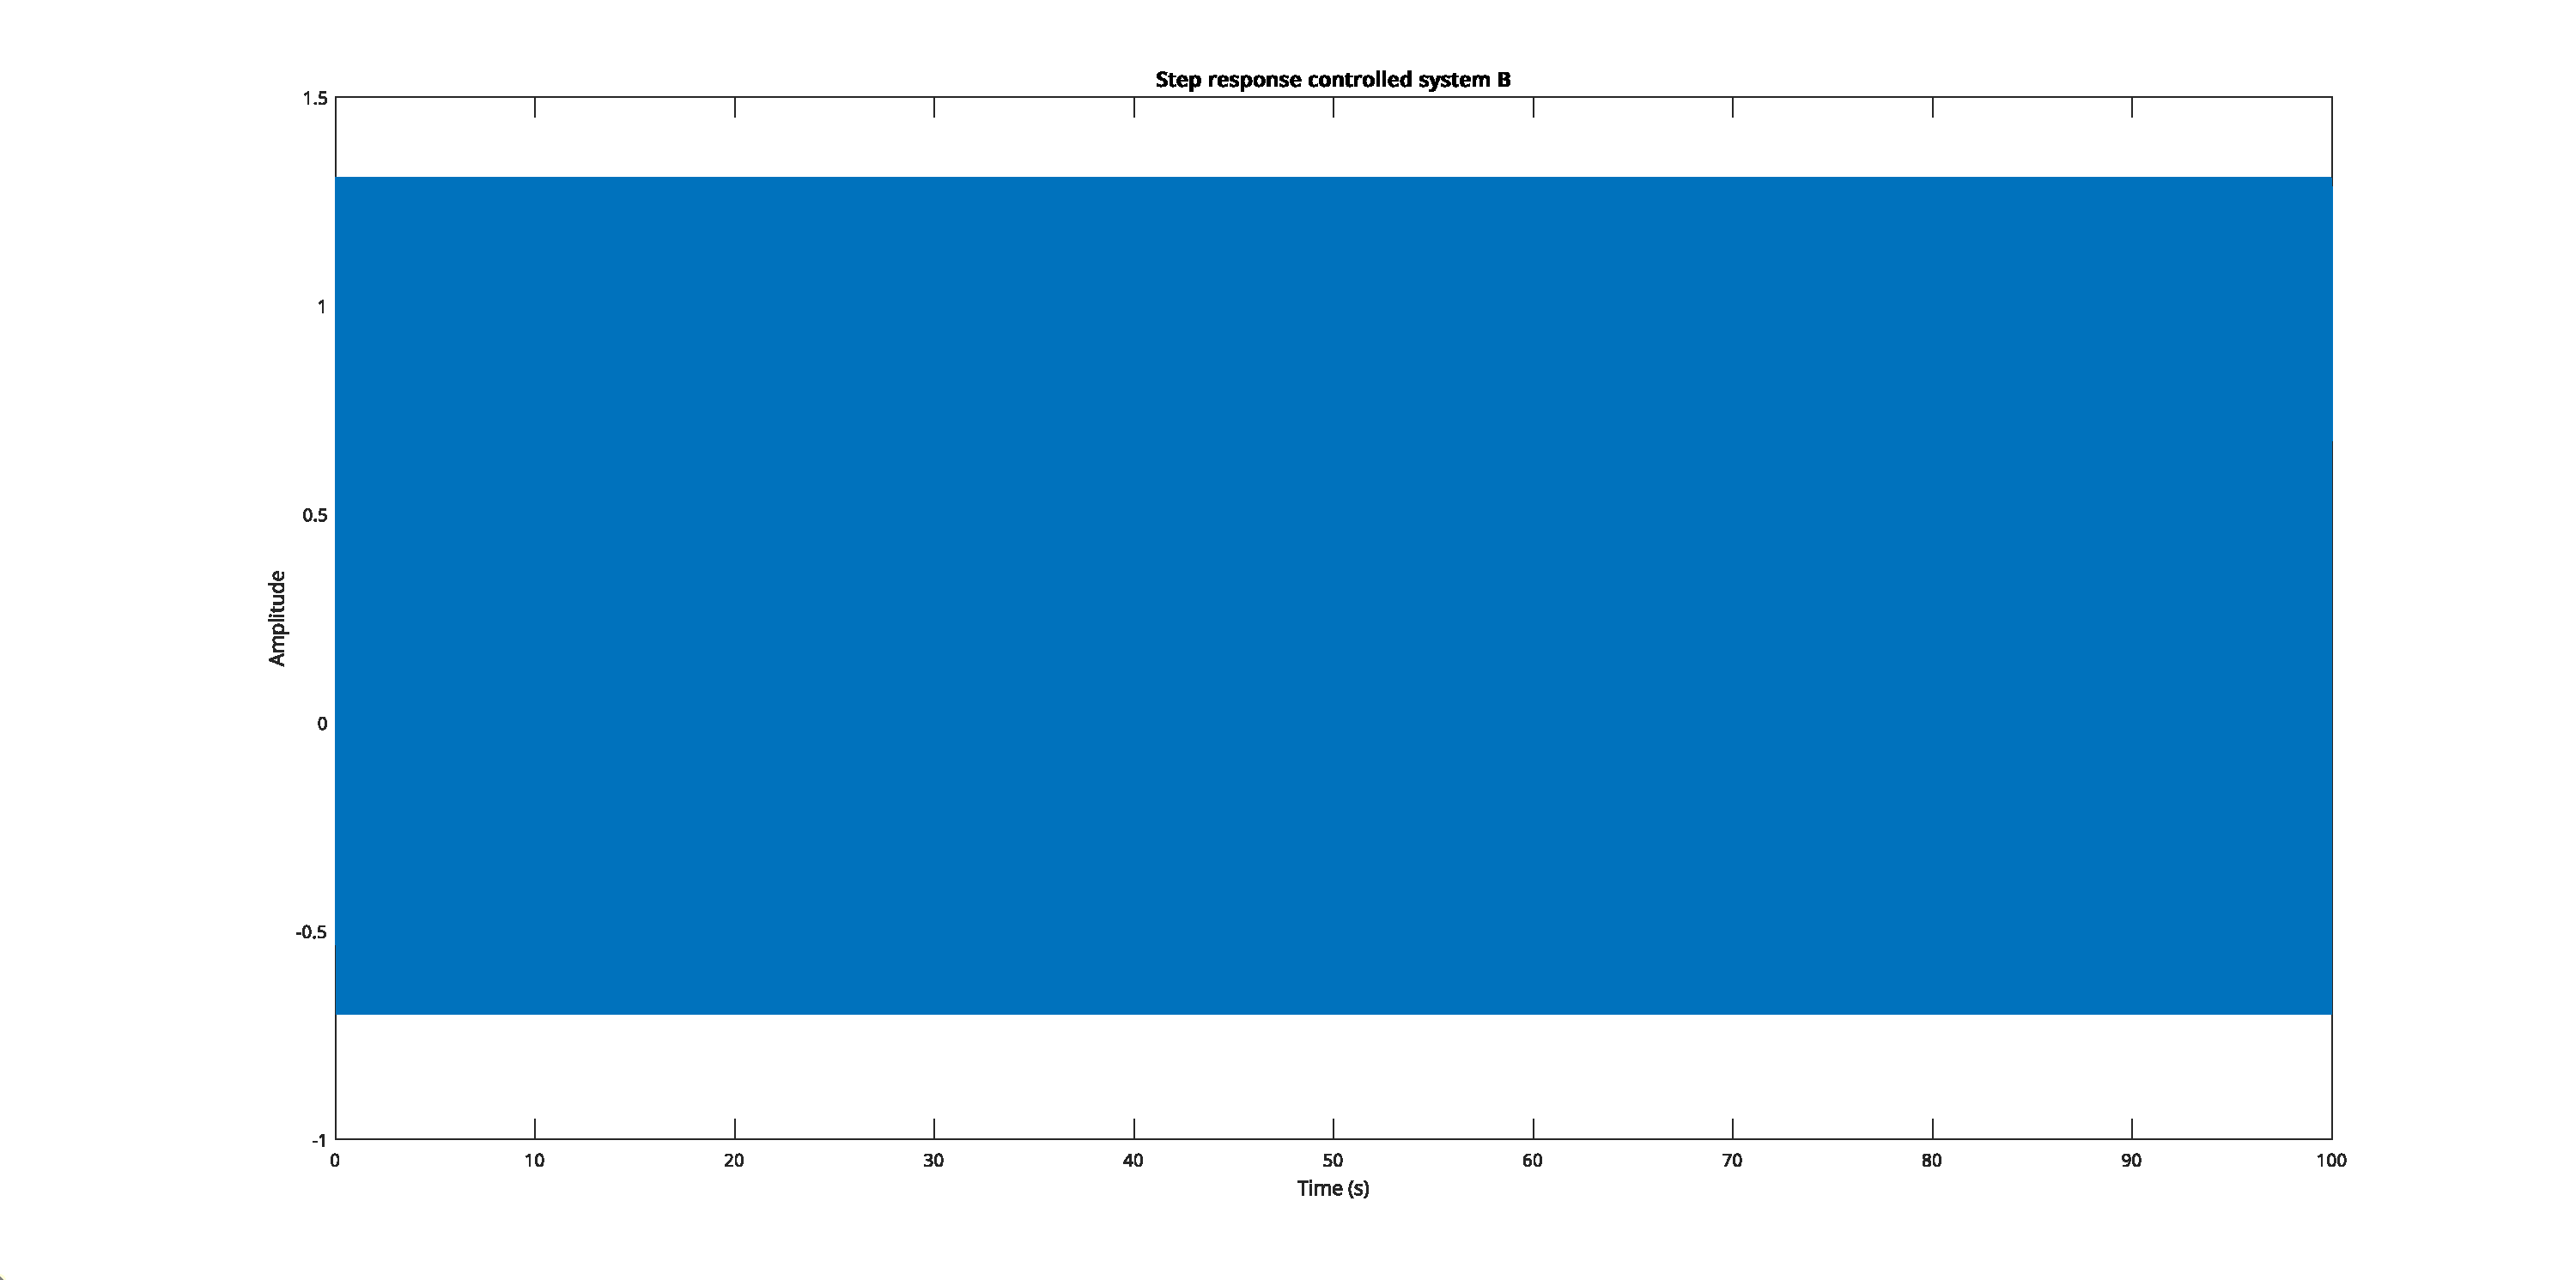
\includegraphics[width=1\linewidth]{stepControlledSystemBLong}
					\caption[step marginal system B long]{long time period}
					\label{fig:stepControlledBLong}
				\end{subfigure}
				\caption{Marginally stable P controlled system B}
				\label{fig:stepControlledB}
			\end{figure}
			
		\subsection{Tuning the system to be critically damped}
			Tuning the system to be critically damped turned out to be more difficult than it appeared at first sight. A typical sign of this type of damping is that we get no overshoot, as we take the most direct path to stability. When we try to dial in the right settings for our P-gain, we see that we keep on having an overshoot. This happens even if we have a large value for our gain. For example when we use the value \num{50000}, we still get an overshoot of 0.0047 .  While we could go further and reduce the overshoot to 0, this would be unproductive as the gain has already exceeded realistic values. 
	\newpage
	\section{Question 4: Control loop for system A}
		\subsection{Layout for the controller}
			\label{sec:PIDcontrollerLayout}
			The unknown model A has been wrapped by a PID controller as seen in figure \ref{fig:PIDcontrolledSystemA}. Here, we see a few elements which are new compared to the P controller in section \ref{sec:PcontrollerSystemB}, we have a time delay, which is set to \num{0} for now. The controller itself is also a bit more complex, it can be seen in figure \ref{fig:PIDcontrollerLayout}. 
			\begin{figure}[h]
				\centering
				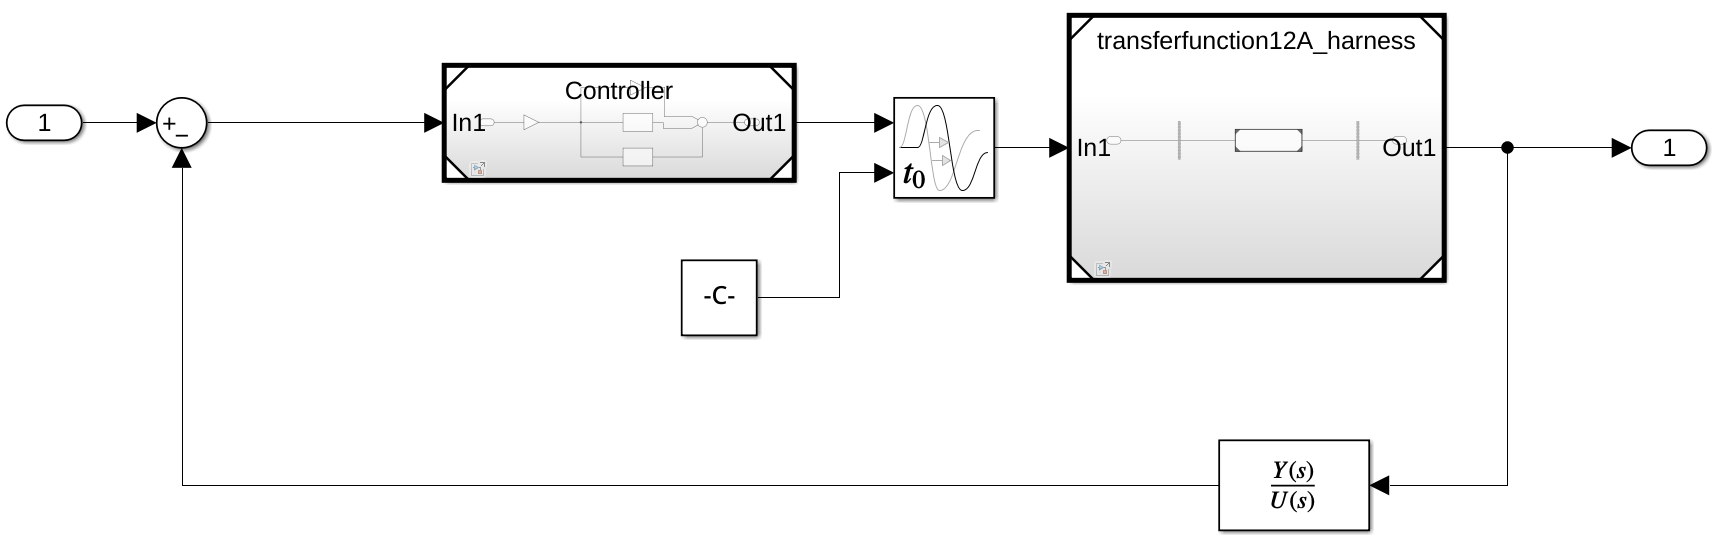
\includegraphics[width=0.7\linewidth]{PIDcontrollerSystemA}
				\caption[PID controller system A]{PID controller for system A}
				\label{fig:PIDcontrolledSystemA}
			\end{figure}
			
			\begin{figure}[h]
				\centering
				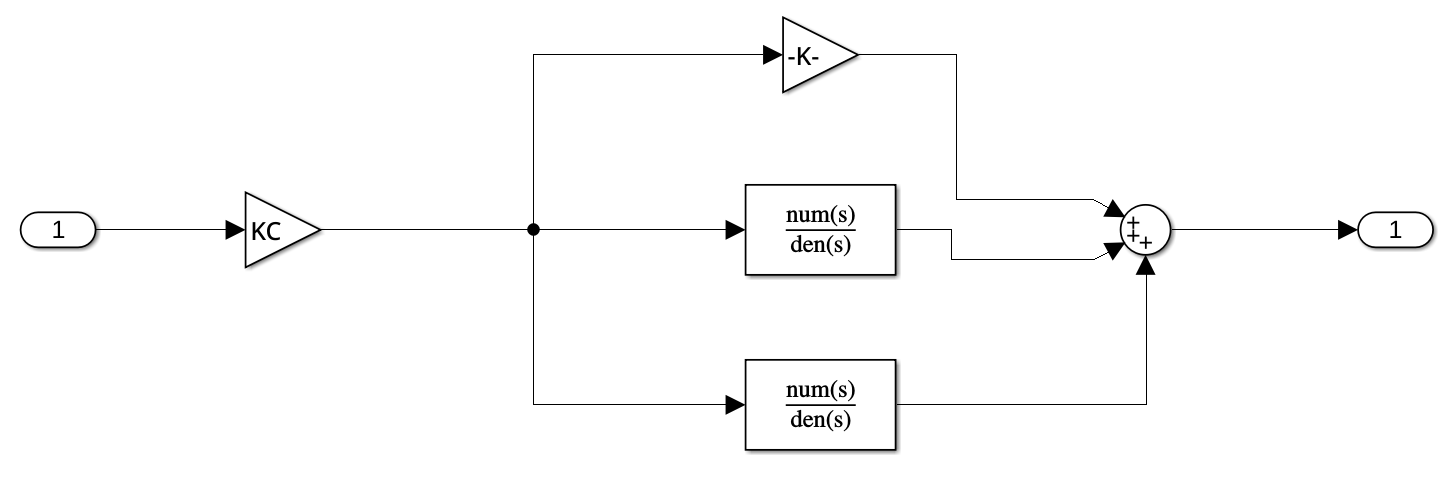
\includegraphics[width=0.7\linewidth]{PIDcontrollerLayout}
				\caption[PID controller structure]{PID controller structure}
				\label{fig:PIDcontrollerLayout}
			\end{figure}
		\subsection{Tuning the controller}
			The controller was tuned using the methods seen in the exercise session for this course. This lead to the following values: $K_C = 70$, $T_I = 0.02$ and $T_D = 0$. 
			\begin{figure}[h]
				\centering
				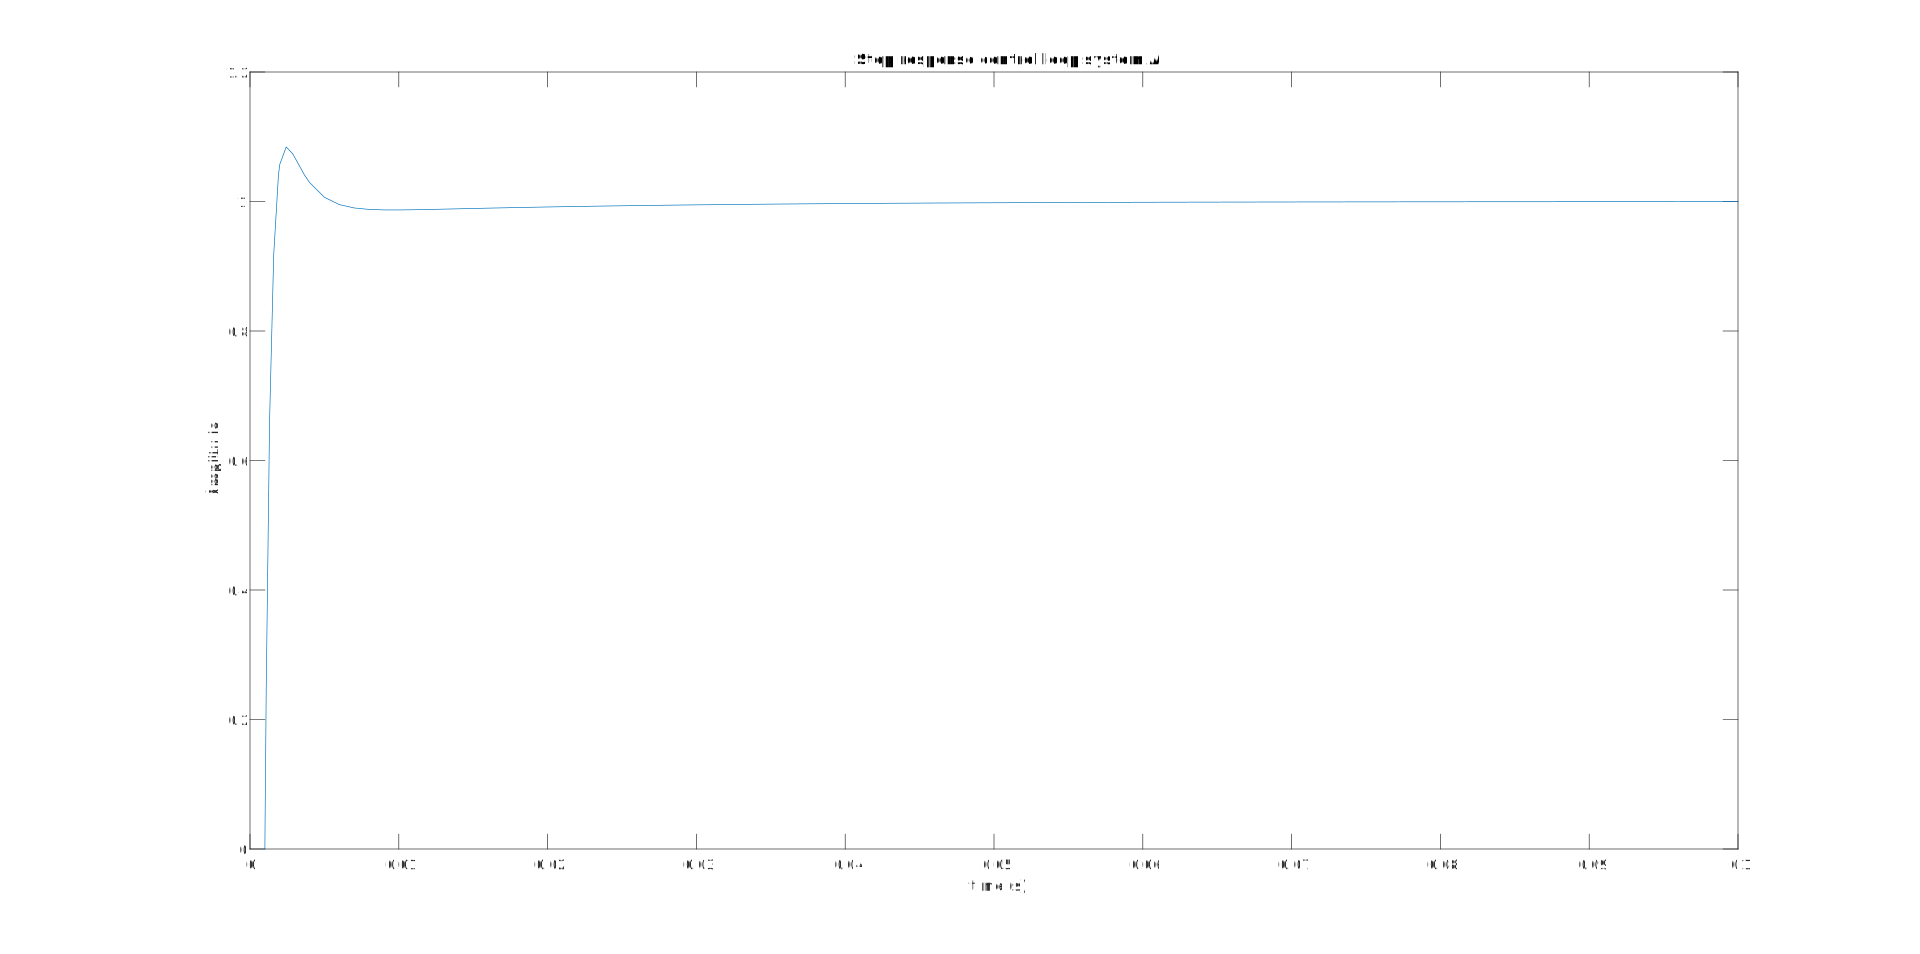
\includegraphics[width=0.7\linewidth]{stepControlledSystemA}
				\caption[Step controlled system A]{Step response for controlled system A}
				\label{fig:stepControlledSystemA}
			\end{figure}
			
		\newpage
		\subsection{Discussion}
			The PID controller is within the requirements set in the assignment. We see an overshoot of about 8.4424, which is within specifications. Furthermore, the system reaches steady state within 0.0044 . An important note to make here, is that we don't have any D action. This is because we don't really see any major oscillations in our step response, so we don't need to filter them out.
	\newpage	
	\section{Question 5: Control loop for system A with delay}
		\subsection{Layout for the controller}
			The set-up for this controller is very much the same as in section \ref{sec:PIDcontrollerLayout}. The only difference is that we now have a time delay. 
			
			
		\subsection{Tuning the controller}
			The controller was tuned using the methods seen in the exercise session for this course. This lead to the following values: $K_C = 0.05$, $T_I = 0.001$ and $T_D = 0$. The system is tuned for a time delay at which it becomes marginally stable, for more details see section \ref{sec:MaxDelay} \\
			
			\begin{figure}[h]
				\centering
				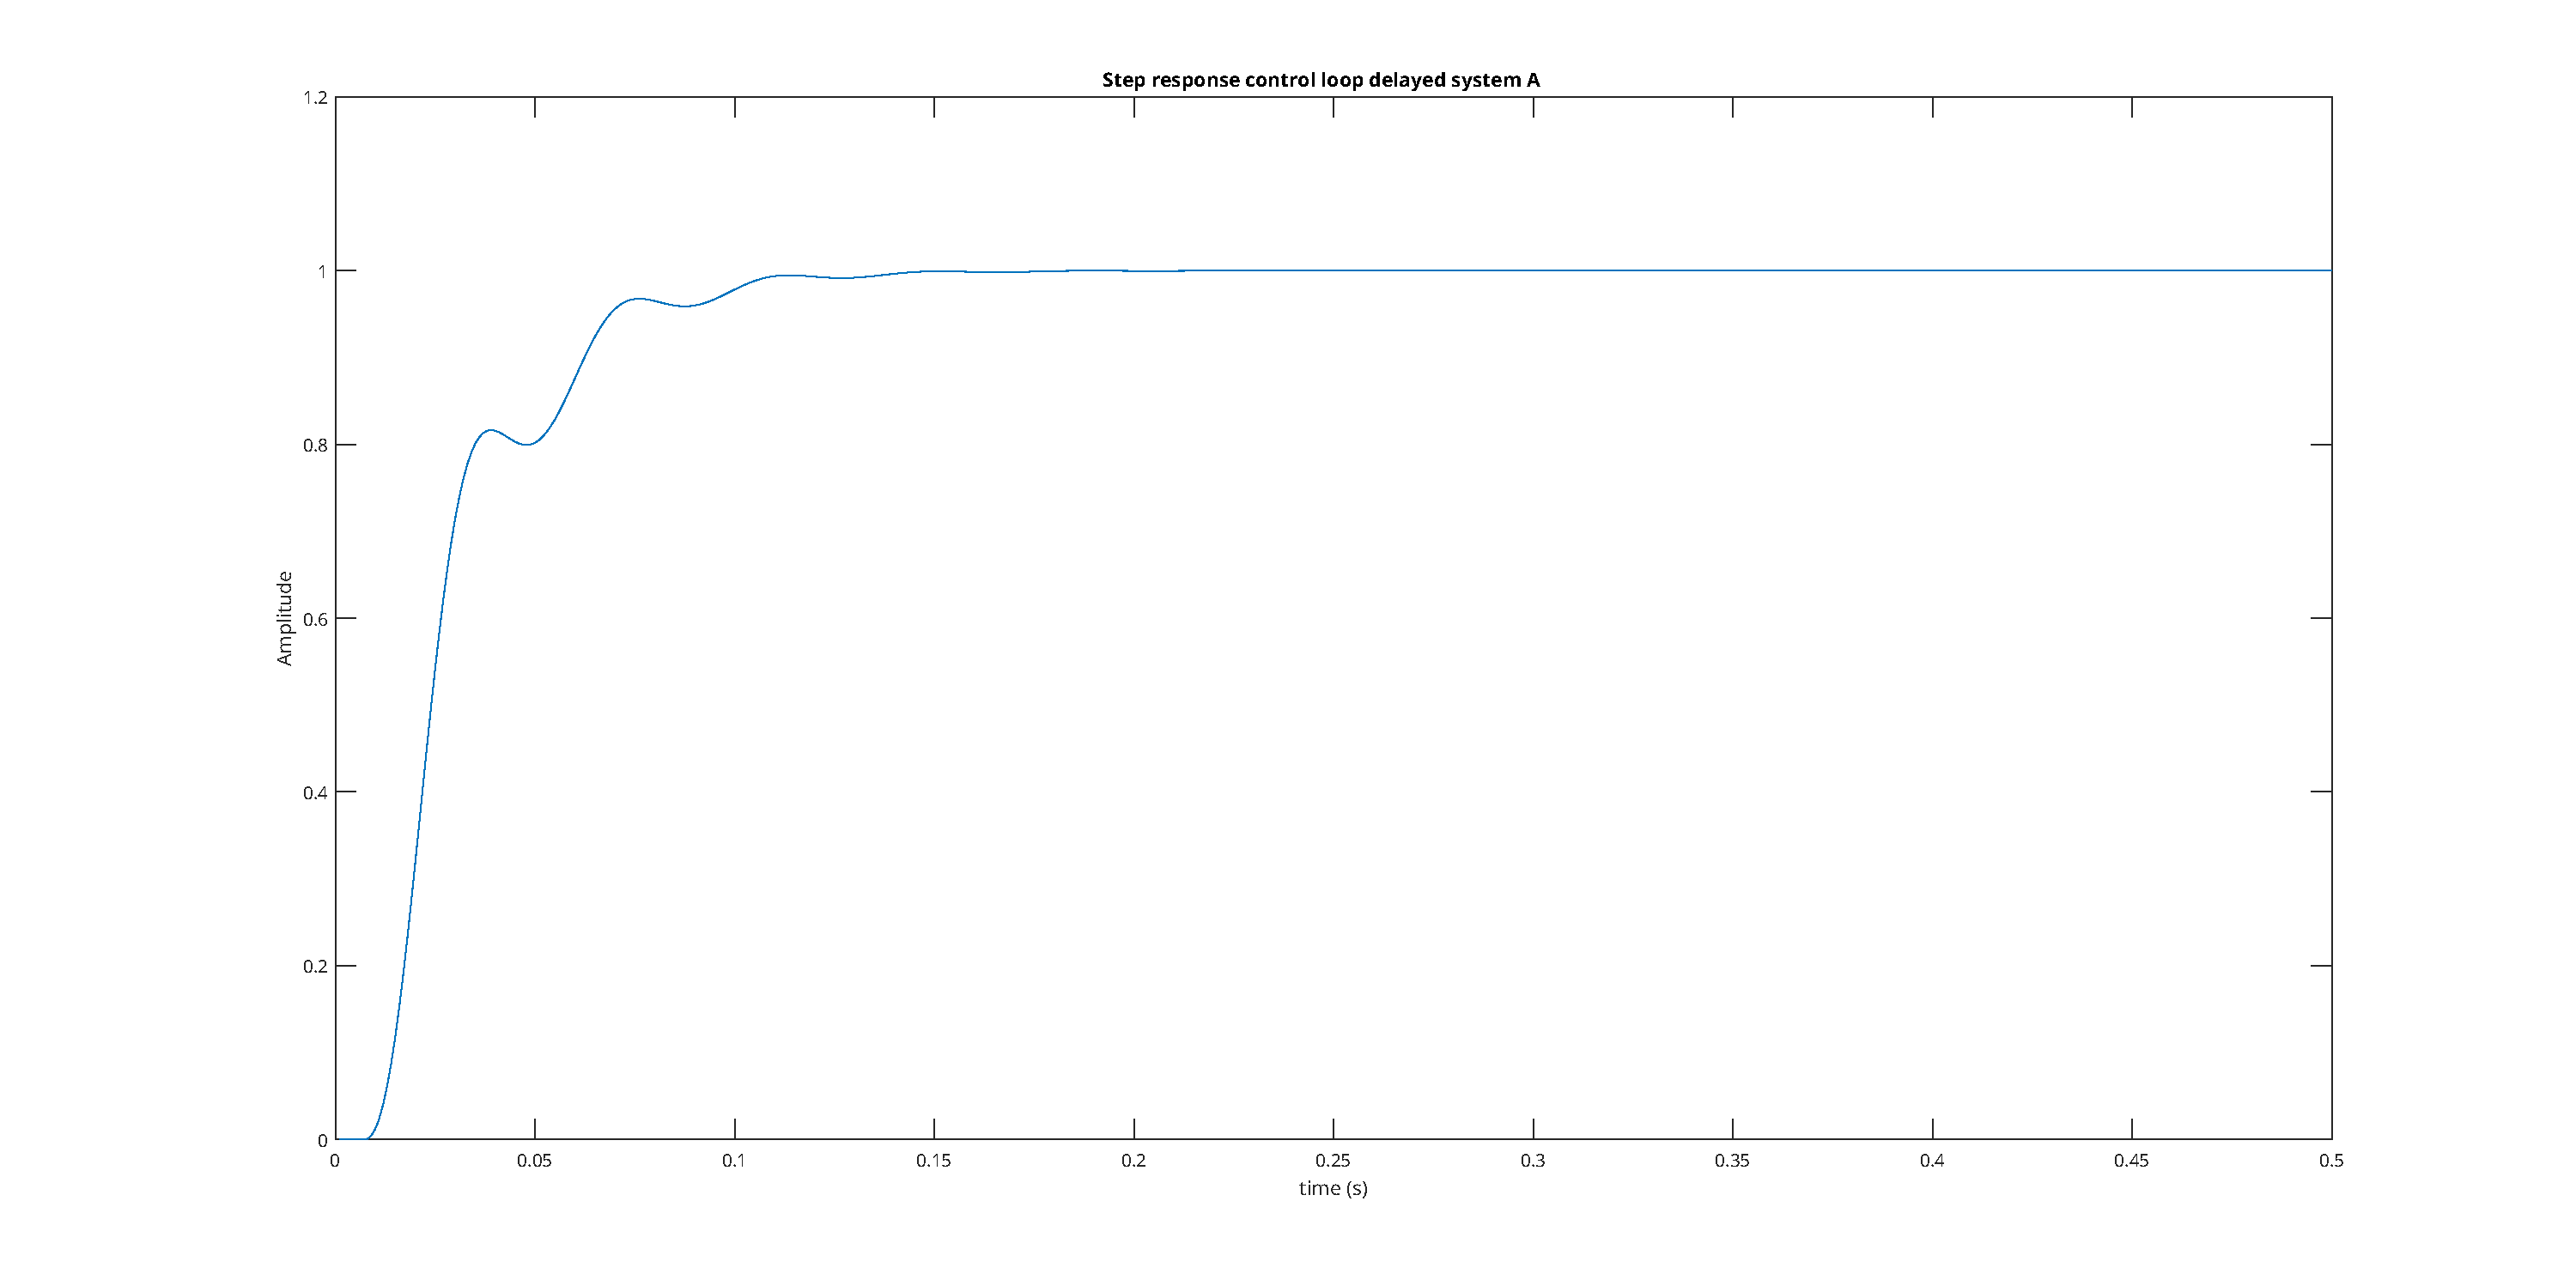
\includegraphics[width=0.7\linewidth]{stepDelayedControlledSystemA}
				\caption[Step delayed controlled system A]{Step response for delayed controlled system A}
				\label{fig:stepDelayedControlledSystemA}
			\end{figure}
			This time around, we see worse performance than with a system which has not been pushed to the edge of stability. We do not have overshoot, but we do take a lot longer to reach steady state (about 0.1 seconds). We also see a lot more oscillations, however, it is not possible to negate this with D action. 
		\subsection{Maximal delay}
			\label{sec:MaxDelay}
			Calculating the maximal delay can simply be done by applying the procedures and formulas seen in the theory lectures of this course. The calculation below shows how to derive the maximal delay for system A before it becomes unstable. Here the values for $\varphi$ and $\omega$ are the ones associated with the phase margin calculated in section \ref{sec:StabilitySystemA}. 
			\begin{align*}
				\varphi &=  \frac{-180}{\pi}t_d\omega\\
				t_d &= \frac{\varphi\pi}{-180\omega}\\
				t_d &= \frac{80\cdot\pi}{-180\cdot 216}\\
				t_d &= 0.00646
			\end{align*}
\end{document}